\documentclass[draft,ms]{agujournal2019}

\usepackage{url} %this package should fix any errors with URLs in refs.
\usepackage{amsmath}
\usepackage{graphicx}
\usepackage{epstopdf}
% \epstopdfDeclareGraphicsRule{.pdf}{png}{.png}{convert -density 40 #1 \OutputFile}
% \DeclareGraphicsExtensions{.png,.pdf}
\usepackage{upgreek}
\usepackage{subcaption}
\usepackage{bm}
\usepackage{float}
\usepackage{multirow}
\usepackage{enumitem}

\usepackage[inline]{trackchanges} %for better track changes. finalnew option will compile document with changes incorporated.
\usepackage{soul}
\linenumbers

\draftfalse


\journalname{Journal of Advances in Modeling Earth Systems (JAMES)}


\begin{document}

%TC:ignore
\title{Snow equi-temperature metamorphism on 3D micro-tomography images using a phase-field model: prediction of microstructural and physical properties}
\textit{Application of a phase-field model on micro-scale snow equi-temperature metamorphism: prediction of microstructural and physical properties}


\authors{L. Bouvet\affil{1,2}, N. Calonne\affil{1}, F. Flin\affil{1}, and C. Geindreau\affil{2}}

\affiliation{1}{Univ. Grenoble Alpes, Université de Toulouse, Météo-France, CNRS, CNRM, Centre d’Études de la Neige, 38000 Grenoble, France}
\affiliation{2}{Univ. Grenoble Alpes, CNRS, Grenoble INP, 3SR, Grenoble, France}

\correspondingauthor{Lisa Bouvet}{lisa.bouvet@univ-grenoble-alpes.fr}

\begin{keypoints}
\item A phase-field model of mean curvature flow is applied on the curvature-driven process of sublimation-deposition describing equi-temperature metamorphism.% and is used on tomographic samples
\item The model is calibrated through the condensation coefficient parameter by fitting experimental and simulated data at -2$^\circ$C.
\item Equi-temperature metamorphism evolution is predicted on a large range of snow microstructures. Microstructural and physical properties are computed and analyzed.
\end{keypoints}


\begin{abstract}

Representing snow equi-temperature metamorphism (ETM) is key to model the evolution and properties of the snow cover. Recently, a phase-field model describing the mean curvature flow on 3D microstructures was proposed \cite{bretin_phase-field_2019}. In the present work, this model is used to simulate ETM at the pore scale, considering the only process of moving interfaces by sublimation-deposition driven by curvatures. We take 3D micro-tomographic images of snow as input in the model and obtain a time series of simulated microstructures as output. Relating the numerical time, as defined in the model, to the real, physical time involves the condensation coefficient, a poorly-constrained parameter. A calibration step was thus done;  we fit simulated microstructures to experimental ones, matching the evolution of the specific surface area (SSA) during ETM at  -2°C.  A value of $(9.8\pm0.7)10^{-4}$ is obtained and used in all the following simulations. The calibrated model enables to well reproduce an independent time series of ETM at -2°C in terms of SSA, covariance length, and mean curvature distribution. Finally, we use the calibrated model to investigate the effect of ETM on four different snow microstructures. As an interesting preliminary result, we observe an enhancement of the structural anisotropy in the case of initially anisotropic microstructures. Also, the potential of such model to provide predictions of effective properties of snow under ETM is illustrated. The evolution of the transport properties (thermal conductivity, vapor diffusion, permeability) is presented and follows current parameterizations.

\end{abstract}

\section*{Plain Language Summary}

Snow on the ground is a skeleton of ice and air that evolves continuously under different environmental constraints. Among them, equi-temperature metamorphism (ETM) refers to the smoothing and rounding of the snow structure under the effect of curvature differences at the ice grain surface. It is one of the main mechanisms of snow evolution and its correct representation is crucial. Here, we use a mean curvature flow model, describing smoothing of 3D microstructures, to simulate ETM of snow. 3D micro-tomographic images of snow samples are used as input; the output is a time series of 3D images showing ETM evolution. The ETM rate is classically driven by the condensation coefficient. This parameter is however still poorly-constrained. We estimate it by fitting the model to experimental data of ETM at -2$^\circ$C. A value of $(9.8\pm0.7)10^{-4}$ is derived. Good agreement is reported when comparing the fitted model to an independent experimental time-series. Finally, we model ETM for four different snow microstructures. The simulated images are then used to predict structural properties and macro-scale transport properties evolution.
Overall this work presents promising tools for snow metamorphism study and the development of predictive means for large scale snow model. 

\section{Introduction}
\label{sec:intro}
Dry snow laying on the ground is a complex material made of an ice skeleton in an air matrix that undergoes continuous transformations. Especially, snow evolves through processes of mass redistribution due to thermodynamic mechanisms called snow metamorphism. Different types of snow metamorphism take place depending on the temperature and humidity conditions as well as on the snow microstructure itself. Considering metamorphism is key as it impacts snowpack physical properties, including mechanical properties involved in avalanche processes or thermo-physical properties that drive the surface energy budget of snowpacks \cite{lehning_physical_2002, vionnet_detailed_2012}.\\

Equi-temperature metamorphism (ETM), also referred to as isothermal metamorphism, occurs in snow in quasi-isothermal conditions and is driven by curvature gradients at the ice-air interface. Low curvature ice surfaces have a lower saturation water vapor density than the high curvature ones. Those curvature gradients lead thus to gradients of saturation vapor density causing vapor transfer across the pores (e.g. diffusion) as well as phase changes (sublimation and deposition). Ice sublimates on higher curvature surfaces and  water vapor deposits on lower curvature surfaces. 

The overall structure of snow gets rounder, coarser, and more sintered \cite{colbeck_thermodynamics_1980}. These morphological changes come together with mechanical grain rearrangement leading to snow settling. The resulting type of snow is referred to as rounded grains (RG) by \textit{The International Classification for Seasonal Snow on the Ground} \cite{fierz2009international}. Equi-temperature metamorphism is constantly taking place in snow but at different levels of intensity. The higher the contrast in curvature and the higher the snow temperature, the more active the equi-temperature metamorphism. In the presence of high temperature gradients, the influence of curvature effects becomes insignificant as the effect of the temperature gradient metamorphism (TGM) predominates.\\

Modeling the physical processes of metamorphism at fine scale requires the  description of the snow microstructure and its evolution (moving interfaces) as well as water vapor transport across the microstructure. Models can be applied on simplified geometry, as in  \citeA{miller_microstructural_2003} who considered a 2D regular network of spherical grains. They can also take as input real snow microstructure, for example 3D images of elementary representative volume (REV) of snow obtained from micro-tomography ($\upmu$CT). To enable micro-scale 3D modeling, different hypothesis can be used, describing kinetics at the interface, with or without vapor diffusion and settling. \citeA{flin_full_2003} considered fully curvature-driven ETM based on the kinetic limited assumption, and simulated it with an iterative method on 3D tomographic images. Comparisons between modeled and experimental microstructures were also shown. \citeA{vetter_simulating_2010} used a Monte-Carlo algorithm to simulate the isothermal metamorphism with the kinetic limited assumption and implemented a simple gravity model to account for settling. They obtained consistent results with observations although the model rely on experimental fitting.\\
Recently, phase-field models have been developed to handle the numerical cost and complexity of 3D micro-scale models \cite{kaempfer_phase-field_2009, granger_physique_2019, bretin_phase-field_2019}. \citeA{kaempfer_phase-field_2009} suggested a phase-field model for snow metamorphism considering interface kinetics and diffusion. They were pioneers with the phase-field method applied to snow metamorphism, and their results are consistent with observations. However, evaluations are qualitative and limited only on one temperature gradient case, mainly because of the numerical cost of the model. 
\citeA{bretin_phase-field_2019} developed a very efficient phase-field multi-phase growth model and applied it to curvature-driven interface evolution, which could be relevant for ETM.\\
Modeling the physics of snow growth classically relies on a condensation parameter $\alpha$ \cite<e.g.,>{ flin_full_2003,libbrecht2005physics, kaempfer_phase-field_2009}. This parameter embodies the surface physics that governs how water molecules are incorporated into the ice lattice and is thus key to model metamorphism. The $\alpha$ coefficient ranges from 0 to 1. One can think of $\alpha$ as a sticking probability, equal to the probability that a water vapor molecule striking the ice surface becomes assimilated into the crystal lattice \cite{libbrecht2005physics}. However, it is still poorly understood and quantified, notably because of its complex dependencies to temperature, humidity and crystalline orientation. Numerous values can be found in the literature, ranging from 10$^{-3}$ to 10$^{-1}$ \cite<e.g.,>{libbrecht_measurements_2013}. The large uncertainty on this coefficient is one of the main limiting factor for metamorphism models accuracy.\\
%
To evaluate 3D models, simulated images are compared to experimental data through microstructural properties that can be calculated on 3D microstructures. Specific surface area (SSA), growth speed, ice thickness and mean curvature were used in previous studies \cite{flin_full_2003, vetter_simulating_2010}. In \citeA{kaempfer_phase-field_2009}, the model results are compared to a 1D pseudo-analytical case using the growth speed variable. Another way of evaluation, not explored yet, could be based on macroscale properties, which can also be calculated on simulated 3D images \cite<e.g.,>{kaempfer2005microstructural, courville2010lattice, srivastava2010observation, calonne_numerical_2011, calonne_study_2014}. It would enable comparison with well established regressions and models from literature.\\
%
% In this article, we apply the phase-field model of \citeA{bretin_phase-field_2019} on the curvature-driven snow equi-temperature metamorphism usable on $\upmu$CT images. We calibrated the model by deriving a single value of the condensation coefficient using an experimental equi-temperature series. This calibration has been evaluated on an independent ETM series. The model has been used to predict ETM on a representative range of 3D microstructures. Those results are shown along with microstructural properties and transport properties, which are analyzed and compared to current models and parameterizations. 
The paper is organized as follows. The model and the tools used for snow analysis are shown along with the model calibration in section \ref{sec:method}. Evaluation of the calibrated model and ETM prediction for different snow microstructures are investigated in section \ref{sec:results}. Section \ref{sec:disc} discuss in details the model artefacts and the different results of the paper. Finally, section \ref{sec:conclusion} concludes the manuscript with a summary. 

\section{Method}
\label{sec:method}
\subsection{Model}
\label{subsec:model}


\begin{figure}
    \centering
    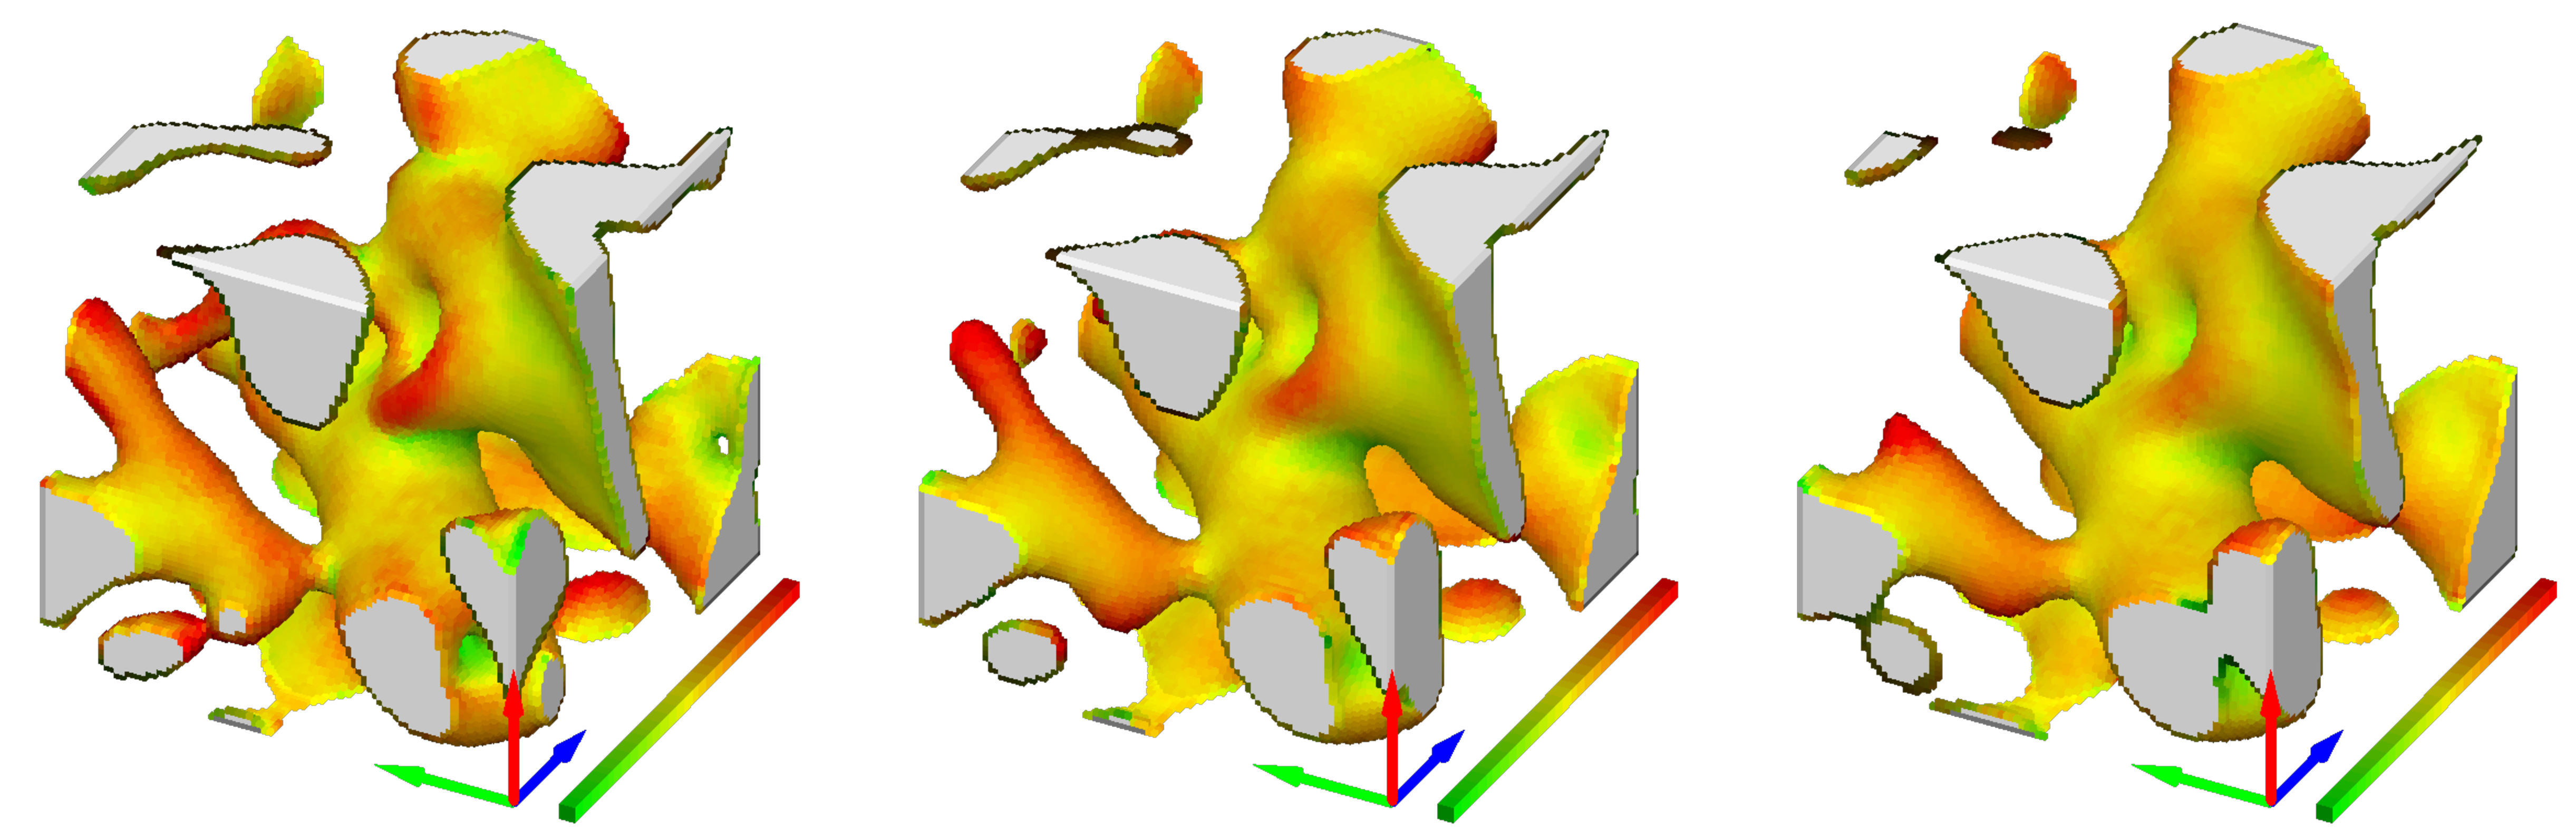
\includegraphics[width=\linewidth]{Figures/eboni_sous_volumes_simu.pdf}
    \caption{3D representation of a tomographic snow sample from \protect\citeA{hagenmuller_motion_2019} under the ETM model Snow-3D after 0, 8 and 16 days at -2$^\circ$C. Concave surfaces are shown in green and convex surfaces in red according to the curvature map of \protect\citeA{ogawa2006representation}.}
    \label{fig:eboni_sous_volume}
\end{figure}

%PHASE FIELD ET MODELE NUMERIQUE
%\color{blue}
The phase-field model of \citeA{bretin_phase-field_2019} simulates a multi-phase medium evolving under mean curvature flow and volume conservation of each phase. This flow is defined by an interface evolution where the normal velocity $v_n$ is proportional to the local interface curvature C. The model minimizes local curvatures while keeping constant the average of the sample mean curvature. The morphological transformation induced by the mean curvature flow can be interpreted as ``smoothing" surfaces and seems suited to model ETM as similar features are encountered. 

% APPLICATION A LA NEIGE (EQUATIONS ETC)
We apply the model of \citeA{bretin_phase-field_2019} to ETM. This implies that we assume the kinetic-limited metamorphism: interface growth velocity depends on the interface kinetic through a condensation coefficient but does not depend on the vapor transport in the pore space. The latter is considered instantaneous, so that vapor density in air is constant and at equilibrium with temperature and with the ambient sample mean curvature. Vapor transport processes in air (diffusion) is thus not described. Also, temperature is considered isotropic and constant. Finally, the model does not include any mechanics and the settling of the ice grains is thus not represented here.\\

Under those conditions, ETM is classically described by the following set of equations \cite<e.g.>{flin_full_2003, kaempfer_phase-field_2009}:  \
\begin{subequations}\label{eq:hertz_knu}
\begin{align}
v_{n} &= \alpha v_{\mathrm{kin}} \frac{\rho_{vs}^{\mathrm{amb}} - \rho_{v s}^{\Gamma}}{\rho_{v s}^{ \Gamma }}\quad \text{on}\ \Gamma\text{,} 
\end{align}
\begin{align}
v_{\mathrm{kin}} &= \frac{\rho_{v s}^{\mathrm{ref}}}{\rho_i}\sqrt{\frac{k T}{2 \pi m}} % vérifier la formulation de vkin ?
\end{align}
\end{subequations}

\begin{subequations}
\begin{align}
\label{equ:gibbsa}
    \rho_{vs}^{\mathrm{amb}}=\rho_{vs}^{\mathrm{ref}}\ e^{d_0 C^{\mathrm{amb}}}
\end{align}
\begin{align}
\label{equ:gibbsb}
    \rho_{vs}^{\Gamma}=\rho_{vs}^{\mathrm{ref}}\ e^{d_0 C} \quad \text{on}\ \Gamma\text{,} 
\end{align}
\end{subequations}

\noindent Equation \eqref{eq:hertz_knu} is the Hertz-Knudsen equation. The velocity normal on the interface and oriented toward the air $v_n$ is related to the difference between the ambient saturation vapor density in the pores $\rho_{vs}^{\mathrm{amb}}$ and the saturation vapor density at the interface $\rho_{vs}^{\Gamma}$.\\

\noindent Equation \eqref{equ:gibbsa} and \eqref{equ:gibbsb} are the Gibbs-Thomson relation applied to the ambient saturated vapor density in the pores $\rho_{vs}^{\mathrm{amb}}$ in equilibrium with the whole sample mean curvature $C^{\mathrm{amb}}$ and applied to the interface saturated water density $\rho_{vs}^{\Gamma}$ at an interface of local curvature $C$. It describes dependencies between saturation vapor density and curvatures using the capillary length $d_0 = \lambda a^3/(k T)$ (m) \cite{kaempfer_phase-field_2009}.\\ 
  
 \noindent $\rho_{vs}^\mathrm{ref}$ is the saturation vapor density in air above a flat surface. It has been largely studied, and can be determined as a function of the temperature using one of the existing parameterizations. We use the formulation of \citeA{gofflow} which is appropriated for our range of temperature and can be found in \citeA{murphy2005review}. All the variables are presented in Table \ref{tab:variables}.

\begin{table}[ht]
\centering
\begin{tabular}{|c|c|c|c|}
\hline \multicolumn{1}{|c} {Symbol} & \multicolumn{1}{|c} { Description } & \multicolumn{1}{|c} { Value, unit } &  \multicolumn{1}{|c|} {Reference} \\
\hline$a$ & mean intermolecular spacing in ice & $3.19 \times 10^{-10}\ \mathrm{m}$ & \cite{petrenko1999physics} \\
$k$ & Boltzmann's constant & $1.38 \times 10^{-23}\ \mathrm{J\ K}^{-1}$ & \\
$m$ & mass of a water molecule & $2.99 \times 10^{-26}\ \mathrm{kg}$ & \cite{petrenko1999physics} \\
$\rho_i$ & density of ice & $917\ \mathrm{kg}\ \mathrm{m}^{-3}$& \\
$\lambda$ & interfacial free energy of ice & $1.09 \times 10^{-1}\ \mathrm{J}\ \mathrm{m}^{-2}$ & \cite{libbrecht1999} \\
$\alpha$ & condensation coeffcient & $10^{-3}\ \mathrm{to}\ 10^{-1}$ & \cite{libbrecht1999} \\
\hline
$\varepsilon$ & interface sharpness parameter & $3$ voxels & \cite{bretin_and_denis_discrete-continuous_2015} \\
$t_{\mathrm{step}}$ & model time step & 0.5 to 8 & \\
$n$ & number of model time steps & 4 to 11 &\\
T & ETM temperature & -2$^\circ$C &\\
\hline
\end{tabular}
\caption{Notations and numerical values of parameters (above) and constants used for the phase-field computations (below).}\label{tab:variables}
\end{table}


The mean curvature flow model of \citeA{bretin_phase-field_2019} is solved with the phase-field method which enables an implicit description of the interface using a function that varies smoothly between different phases. When adapted and applied to ETM with two-phases, air and ice, the phase-field equation can be expressed as:\\
\begin{equation}\label{eq:phase-field}\frac{\partial u}{\partial t}(x, t)= d_0 \alpha v_{\mathrm{kin}} \left(\Delta u(x, t)-\frac{1}{\varepsilon^{2}} W^{\prime}(u)\right)\end{equation}
\noindent with $x$ the position, $t$ the time and $u$ the phase function defined as: \begin{equation}\label{eq:phase-func}
u(x,t) := \frac{1}{2}\left(1-\tanh\left(\frac{s}{2}\right)\right)\frac{d(x,t)}{\varepsilon}
\end{equation}
with $s$ the curvilinear  abscissa, $d$ the distance function from the interface $\Gamma$, $\varepsilon$ the interface sharpness parameter, and $W$ a double-well potential $W(s):=\frac{1}{2} s^{2}(1-s)^{2}$. The distance function is linked to the surface local curvature C by $\Delta d(x) = C$ and to the interface normal speed $v_n$ by $\partial_t d (x,t) = - v_n$. By substituting the physical variables to non-dimensional variables such as: $\Tilde{t} = t \alpha v_{\mathrm{kin}} d_0 / d_x^2 $, $\Tilde{x} = x/d_x$ and $\Tilde{\varepsilon} = \varepsilon/d_x$ with $d_x$ (m) the input image resolution, the canonical dimensionless form of equation \ref{eq:phase-field} is the famous Allen-Cahn equation \cite{bretin_and_denis_discrete-continuous_2015, kaempfer_phase-field_2009}:
% \begin{equation}\label{eq:allen-cahn}\frac{\partial u}{\partial t}(x, t)=\Delta u(x, t)-\frac{1}{\varepsilon^{2}} W^{\prime}(u)\end{equation}
\begin{equation}\label{eq:allen-cahn}\frac{\partial \Tilde{u}}{\partial \Tilde{t}}(\Tilde{x}, \Tilde{t})=\Delta \Tilde{u}(\Tilde{x}, \Tilde{t})-\frac{1}{\Tilde{\varepsilon}^{2}} W^{\prime}(\Tilde{u})\end{equation}

% \begin{figure}
%     \centering
%     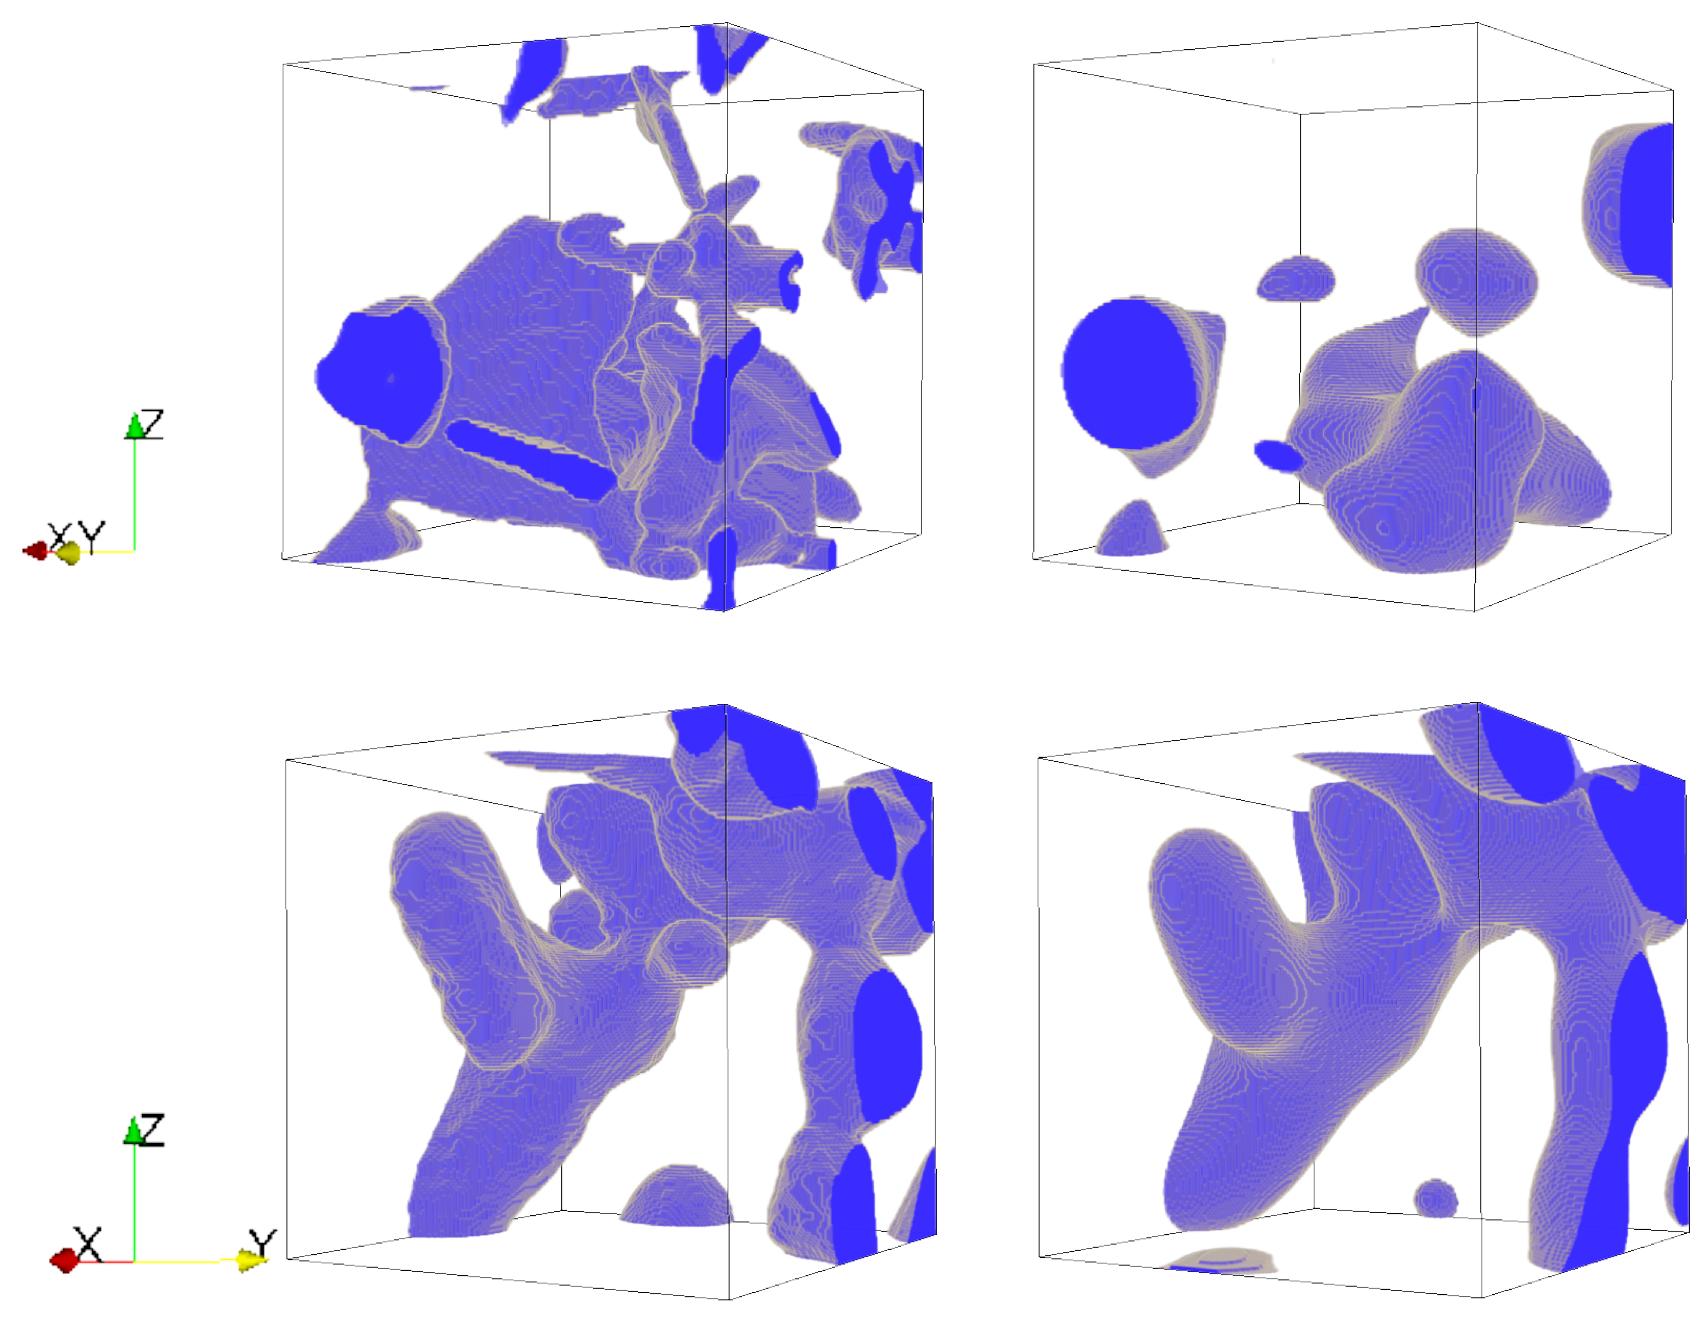
\includegraphics[width=0.7\linewidth]{Figures/disconnections_iso01_iso15.pdf}
%     \caption{Influence of the starting snow type on the disconnections. a) Fresh snow from \protect\cite{flin_three-dimensional_2004} series: initial state (left) and after 40 days of simulation (right) ; b) Sample that underwent 30 days of equi-temperature conditions: initial state (left) and after 40 days of simulation (right) }
%     \label{fig:disco}
% \end{figure}

The equation \eqref{eq:allen-cahn} is the general form of the phase-field equation. In the model another term is added on the form of a Lagrangian multiplier to guarantee the volume conservation \cite<See>{bretin_phase-field_2019}.



The resulting software is called Snow-3D. The model takes as input a 3D binary image of snow microstructure, as illustrated in Figure \ref{fig:eboni_sous_volume}. The output is a series of simulated 3D binary images at different time steps of the simulation. The adjustable parameters are the time step $t_{\mathrm{step}}$, the number of time steps $n$ and the interface sharpness parameter $\varepsilon$. The different ranges used for those parameters in this work are given in Table \ref{tab:variables}. In Figure \ref{fig:eboni_sous_volume} the effect of the curvature-driven evolution is illustrated with ice sublimation on high curvature surfaces and water vapor deposition on low curvature surfaces.

% ARTEFACTS
Finally, corrections were necessary to limit some artefacts of the model. Periodic boundary conditions are applied on the images. It leads to errors in estimating curvature at the image boundaries resulting in very high curvatures. The edges of the simulated images were thus cut off of a certain width (0.6 mm) prior to further analysis. Also, as the model does not simulate gravity, simulations can lead to create ``floating" ice grains,  especially for snow in early stages of metamorphism that undergo significant settling \cite{schleef2014influence}. 
% An example of grain disconnections is shown in Figure \ref{fig:disco}. 
To prevent this non-physical phenomenon, we restrict input simulation to adequate snow microstructures and suppress disconnected ice grains.
% As an example, we loose 6.10$^{-4}$ g of Grad3 sample (0.08 g) during the simulated 75 days of ETM with the SUPPRESSION of disconnected particles. 



\subsection{Calibration} 
\label{subsec:calib}

\begin{table}
\hspace*{-0.5cm}
\begin{tabular}{|c|c|c|c|c|c|}
\hline Reference & ETM stage & Resolution & Dimension & Density & Snow types \\
 &  & ($\upmu$m) &(voxel) & (kg m$^{-3}$) &  \\
\hline 
\cite{flin_three-dimensional_2004} & $84\ \mathrm{days}$, T = $-2^{\circ} \mathrm{C}$ & 4.9 & 512 & 158 & \small{$\mathrm{PP} \rightarrow \mathrm{RG}$} \\
\cite{hagenmuller_motion_2019} & 4 days, $\mathrm{T}=-2^{\circ} \mathrm{C}$ & 7.5 & 450 & 212 & \small{$\mathrm{DF/RG}$} \\
\hline
\end{tabular}
\caption{Experimental equi-temperature series used to calibrate and evaluate the model. The density corresponds to the initial density of the used portion of each series. The snow types separated by an arrow present the initial and final type of the series.}
\label{tab:series_exp}
\end{table}


 The model output is a series of $n$ images separated by a time step $t_{\mathrm{step}}$, without any notion of physical duration. To obtain physical simulation evolution, a calibration step is thus needed.
Considering the non-dimensional time used to deduce the dimensionless equation \eqref{eq:allen-cahn}, the model physical time can be expressed as \cite{bretin_and_denis_discrete-continuous_2015}: 
\begin{equation}\label{equ:alpha}
   t = \frac{\Tilde{t}\ d_x^2}{\alpha v_{\mathrm{kin}} d_0}
\end{equation}
with $t$ the physical time (s) and $\Tilde{t} = t_{\mathrm{step}} \times n$ the simulated time (-). As the only poorly determined parameter, the condensation coefficient $\alpha$ is needed to determine the physical time. To derive a value of $\alpha$, we compare a simulated series with a part of the experimental series of \citeA{flin_three-dimensional_2004} (cf Table \ref{tab:series_exp}) using the time evolution of the SSA parameter. $\alpha$ have been calibrated using the SSA because it is a good scalar descriptor of the microstructure evolution.\\
The series corresponds to 10 tomographic images of snow microstructure showing snow at different time of its evolution in ETM at -2$^\circ$C, from 0 to 84 days. The series used samples that were extruded at different locations of the snow slab for each tomographic scan. The first images of the series of \citeA{flin_three-dimensional_2004} correspond to fresh snow and were not used to avoid grains disconnection issues (Sec. \ref{subsec:model}).\\
The calibration process is schematized in 5 steps in Figure \ref{fig:workflow}. For each selected image of the experimental series taken successively as input: \\
\begin{enumerate}
    \item We used the model Snow-3D to obtain a simulated series composed of 10 images. 
    \item We calculated the SSA temporal evolution of the series during the simulation (Graphs b).
    \item We fitted the SSA of the simulated series (Graph b) to the SSA of the experimental series (Graph a) by adjusting the time axis. More precisely, we scaled the simulation steps to the real time such that they match the experiment best by minimizing the Root Mean Square Error (RMSE) between the two curves (Graph c).   
    \item We used the simulation time and the fitted physical time to derive a value of the condensation coefficient $\alpha$ through the equation \eqref{equ:alpha}. 
\end{enumerate}

\hspace*{-0.2cm}
\begin{figure}
    \centering
    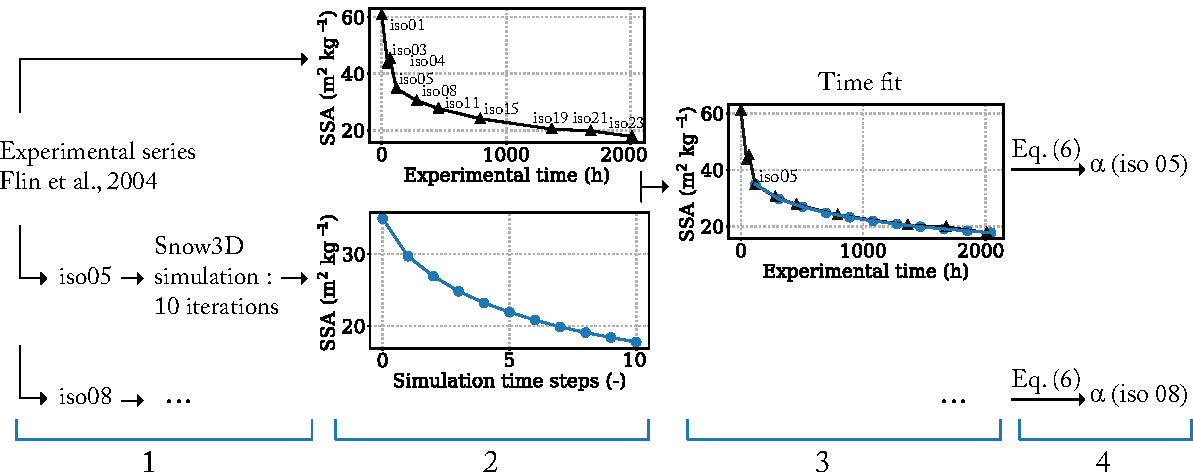
\includegraphics[width = \linewidth]{Figures/workflow_aff.pdf}
    \caption{Workflow of the time calibration approach}
    \label{fig:workflow}
\end{figure}
Those steps have been applied to the image Iso05 (day 5), Iso08 (day 12), Iso11 (day18) and Iso15 (day 33). The last three images of the experimental series (Iso19, Iso21, and Iso23) were not used as they are close in time to the end of the experiment, which prevent a precise estimation of $\alpha$. %It resulted in 4 simulated series composed of 10 images simulating equi-temperature metamorphism from a different input image, i.e. from a different metamorphism stage.
We removed on each side of the simulated image a layer with a thickness equal to the size of two heterogeneities (0.6 mm) before the SSA calculation to avoid edge artefacts while keeping volumes larger than REVs (representative elementary volume) for most of the properties of interest. The average and the standard deviation are calculated on the 4 resulting $\alpha$ coefficients. The resulting condensation coefficient is $\alpha = ( 9.8 \pm 0.7) 10^{-4}$. As the temperature condition of \citeA{flin_three-dimensional_2004} is -2$^\circ$C, the calibrated model can only be used to simulate ETM at -2$^\circ$C. To see the influence of $\alpha$ in the microstructural parameters, we calculated the variation of the microstructural parameters as a function of $\alpha$ variation. In the range of the $\alpha$ derived from the different samples, the parameters such as density, SSA and covariance length (described in Section \ref{subsec:methode_physical_appli}) only have a maximum alteration of 5\%, which is small compared to the physical precision of those parameters. 

\subsection{Computation of snow properties}
\label{subsec:methode_physical_appli}

\begin{table}
\hspace*{-3cm}
\begin{tabular}{|c|c|c|c|c|c|}
\hline Name (Reference) & Metamorphism stage & Resolution & Dimension & Density & Snow types \\
 &  & ($\upmu$m) &(voxel) & (kg m$^{-3}$) &  \\
\hline 
I17 \small{\cite{dumont2017experimental}} & Recent snow & 7.3 & 700 & 147 & \small{$\mathrm{DF}$} \\
TG2 \small{\cite{dumont2017experimental}} & 16 days, $\mathrm{TG}=19\ \mathrm{K}\ \mathrm{m}^{-1}, \mathrm{T}=-5^{\circ} \mathrm{C}$ & 7 & 700 & 254 & \small{$\mathrm{FC} / \mathrm{DH}$} \\
Grad3 \small{\cite{flin2011computations}} & 8 days, $\mathrm{TG}=100\ \mathrm{K}\ \mathrm{m}^{-1}, \mathrm{T}=-5^{\circ} \mathrm{C}$ & 10 & 600 & 372 & \small{$\mathrm{DH}$} \\
7G9m \small{\cite{calonne_study_2014}} & 21 days, $\mathrm{TG}=43\ \mathrm{K}\ \mathrm{m}^{-1}, \mathrm{T}=-4^{\circ} \mathrm{C}$ & 9.7 & 950 & 314 & \small{$\mathrm{DH}$} \\
\hline
\end{tabular}
\caption{Experimental images used as prediction to simulate isothermal metamorphism.}
\label{tab:series_sim}
\end{table}



To characterize our simulated and experimental microstructures, we calculated on our volumes a range of microstructural and physical properties. Those properties are defined and used as in \citeA{calonne_study_2014}.

\noindent \textbf{Microstructural properties}$\quad$ To describe the structure of our snow images at fine scale, we computed microstructural properties on the volumes using counting and normal vectors algorithms. The properties used are:
\begin{itemize}
    \item The snow density $\rho_{\mathrm{s}}$ computed with a simple voxel counting algorithm.
    
    \item The mean curvature MC (mm$^{-1}$), defined as $\mathrm{MC} = \left(C_{min} + C_{max})\right/2$ with $C_{min}$ and $C_{max}$ respectively the minimum and maximum 2-D curvatures at one point of the surface. As those values are computed for each point of the surface, they are represented as statistical distributions. Values near 0 mm$^{-1}$ correspond to flat surfaces, positive values are convex surfaces, and negative values are concave surfaces; the higher the values, the more concave or convex the surfaces \cite{flin_three-dimensional_2004, brzoska2007using, wang2012curvature}. The mean curvature is expressed in terms of occurrence ratio, which gives the percentage of the ice surface area that exhibits a mean curvature located in a particular curvature class.
    % In the Figure \ref{fig:MC} in both histograms the mean decreases towards 0 with iterations, which corresponds to larger and rounded grains. In the downward mean curvature, the asymmetry at the first iterations is explained by the facets (plane surfaces) oriented downward from the TG metamorphism that will get rounder with the isothermal metamorphism model.\\
    
    \item The specific surface area SSA (m$^2$ kg$^{-1}$), defined by the ratio between the total ice surface of a sample and its volume of ice per mass unit: $\mathrm{SSA}=S/V \times \rho_{i}$ \cite{flin2011computations, berryman1998planar}.
    
    \item  The covariance (or correlation) length $l_{c}$, calculated along the x-, y-and z- direction of the images, which provide a characteristic length of the microstructure, corresponding to the characteristic size of heterogeneities. It is used to characterize the basic microstructure geometry \cite{lowe2013general}. 
    
    \item Anisotropy coefficient
    $\mathcal{A}(\star)$, that can be computed for each microstructural and physical property which are computed along 3 dimensions. This coefficient is defined as the ratio between the vertical component over the horizontal one, such as $\mathcal{A}(\star)=\star_{z} / \star x y$. The property is considered isotropic if it exhibits a coefficient close to 1, otherwise the property is anisotropic. For example, $\mathcal{A}(l_c)$ largely above 1 means that the covariance length is higher in the vertical direction than in the horizontal one, and thus describe a structure that is vertically elongated.
\end{itemize}


\noindent \textbf{Macroscale transport properties}$\quad$ The 3D tensor of the effective coefficient of diffusion  $\mathbf{D}$ (m$^2$ s$^{-1}$), of the effective thermal conductivity $\mathbf{k}$ and of the intrinsic permeability  $\mathbf{K}$ (m$^2$) were computed on a set of simulated 3D images. For each property, a specific boundary value problem, arising from a homogenization technique \cite{auriault2009homogenization, calonne2015macroscopic}, is solved on the images applying periodic boundary conditions on the external boundaries of each volume using the software Geodict \cite{thoemen_3d_2008}. The effective diffusion coefficient was computed with an artificial diffusion coefficient of gas in free air set to $D^{\mathrm{air}} =$ 1 m$^2$ s$^{-1}$. In this study, we present the normalized values of the effective diffusion $\mathbf{D} / D^{\mathrm{air}}$ (dimensionless). %These normalized values can be multiplied by the diffusion coefficient of the gas of interest in free air to get the physical, non-normalized values of effective diffusion coefficient of this gas in snow or firn (for example, the diffusion coefficient of vapor in free air, that is $2.036 \times 10^{-5}$ m$^2$ s$^{-1}$ at -10$^\circ$C \cite{massman_review_1998}, could be used to get the effective diffusion coefficient of vapor). 
$\mathbf{K}$ is normalized by the equivalent sphere radius $r_{\mathrm{es}}=3/(\mathrm{SSA} \times \rho_{\mathrm{i}})$ to introduce a dimensionless tensor: $\mathbf{K}\mathrm{^{*}} = \mathbf{K}/r_{\mathrm{es}}^2$  \cite{calonne_3D_2012}.
As the non-diagonal terms of the tensor $\mathbf{D}$, $\mathbf{k}$ and  $\mathbf{K}$ are negligible, we consider only the diagonal terms, i.e. seen as the eigenvalues of the tensors (the image axes $x$, $y$ and $z$ are the principal directions of the microstructure, $z$ being along the direction of gravity). Besides, the tensors are transversely isotropic as the components in $x$ are very similar to the ones in $y$.
In the following, $D$, $k$ and $K$ refer to the averages of the diagonal terms of $\mathbf{D}$, $\mathbf{k}$ and $\mathbf{K}$, respectively. $D_z$, $k_z$ and $K_z$ refer to the vertical components and $D_{xy}$, $k_{xy}$ and $K_{xy}$ refer to the mean horizontal components where $D_{xy} = (D_{x} + D_{y}) /2$, $k_{xy} = (k_{x} + k_{y}) /2$ and $K_{xy} = (K_{x} + K_{y}) /2$. Finally, the anisotropy of the properties is characterized based on the anisotropy ratio $\mathcal{A}(D) = D_z / D_{xy}$, $\mathcal{A}(k) = k_z / k_{xy}$ and $\mathcal{A}(K) = K_z / K_{xy}$ \cite<e.g.>{calonne_study_2014}.


\section{Results}
\label{sec:results}
\subsection{Model evaluation}
\label{Section:Calibration}

\begin{figure}
    \centering
    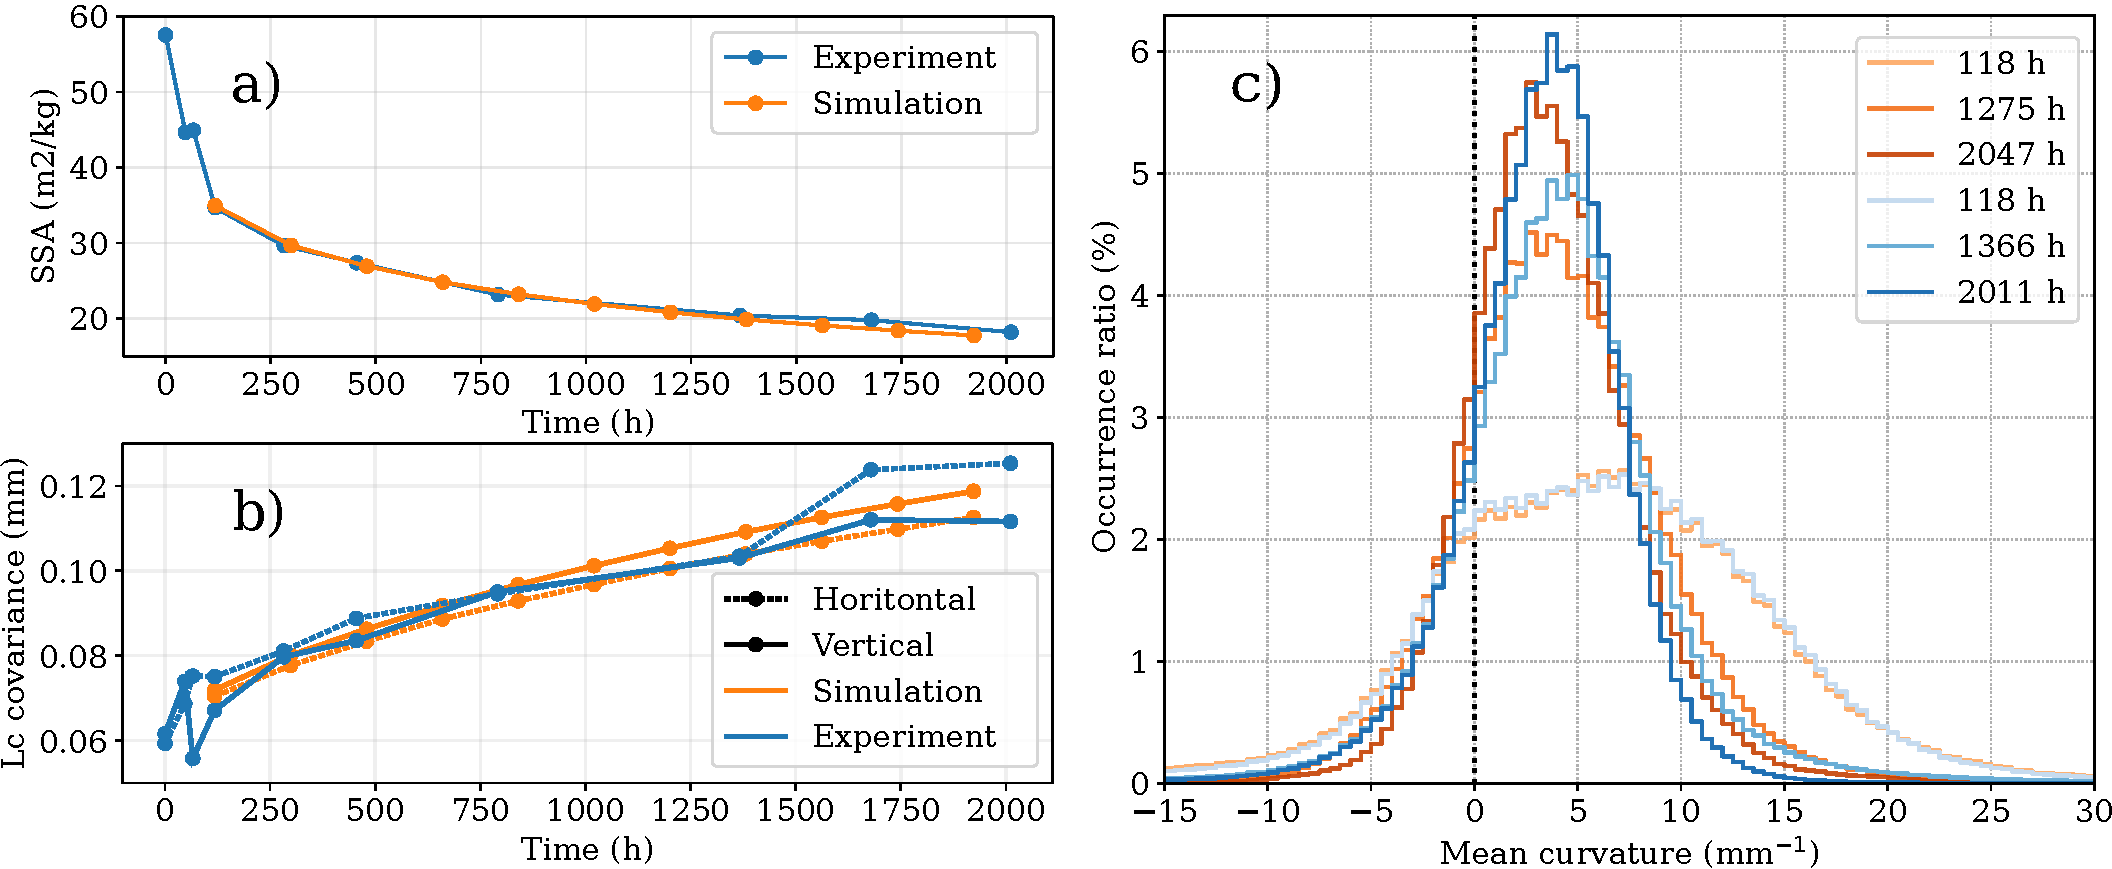
\includegraphics[width=\linewidth]{Figures/flin_evaluation_courbes_lc_ssa_histo.pdf}
    \caption{Comparison between the simulation and the experiment of \protect\citeA{flin_three-dimensional_2004} starting from the iso05 sample. a) SSA ; b) correlation length ; c) mean curvature histograms.}
    \label{fig:flin_evaluation}
\end{figure}

Here, we evaluate the calibrated model by comparing experiments and simulations. We first evaluate the model results with the time series of \citeA{flin_three-dimensional_2004} i.e. the dataset used to calibrate the condensation coefficient required in the model (Sec. \ref{subsec:calib}), using  Iso05 (RG) as initial image. We also use the experimental series of \citeA{hagenmuller_motion_2019} to allow for an independent comparison.\\

The series of \citeA{hagenmuller_motion_2019} (Table \ref{tab:series_exp}) is a 110 h long experiment of equi-temperature metamorphism at -2$^\circ$C with 32 tomographic images. The series was used to study dust particles in snow under temperature gradient and equi-temperature conditions with a dust content of 0.5 mg g$^{-1}$. We assume that dust has little influence on ETM, and to use the images as model inputs, the dust particles were converted to air. Here we focus on the equi-temperature part of the experiment (approx. 70 h of ETM and 20 tomographic images). In the work of \citeA{hagenmuller_motion_2019}, the snow sample was observed with in operando X-ray tomography, meaning than the same sample was scanned at regular intervals. It enables to compare directly simulated and experimental images, unlike the \citeA{flin_three-dimensional_2004} series for which each image corresponds to a different sample.\\

Results of SSA, covariance length and mean curvature for each time series are shown in Figure \ref{fig:flin_evaluation} and \ref{fig:eboni}, respectively. As expected, simulations follow closely the SSA decrease reported in the experiment of \citeA{flin_three-dimensional_2004} (Fig \ref{fig:flin_evaluation}.a).
The RMSE is of $0.58\ \mathrm{m}^2\ \mathrm{kg}^{-1}$ for SSA values evolving from 35 to 18 m$^2$ kg$^{-1}$.
Covariance lengths increase over time from around 0.07 to 0.12 mm. This overall evolution is well reproduced by the model with a small RMSE of $0.005\ \mathrm{mm}$ (Fig. \ref{fig:flin_evaluation}.b). Looking in more details, the snow microstructure gets slightly elongated in the horizontal direction with covariance length about 0.02 mm higher in the horizontal direction than in the vertical one. This is not captured in the simulations in which differences between the lengths in both directions remains rather constant over time and do not exceed 0.005 mm. We should however keep in mind that the experimental data do not only reflect a time evolution but also the spatial variability of the snow layer monitored in \citeA{flin_three-dimensional_2004}, the latter being not considered in simulations, as explained in Section \ref{sec:method}. This might explain the small disagreement observed in correlation lengths.
Finally, the mean curvature distribution presented in Figure \ref{fig:flin_evaluation}.c allows to qualitatively compare the evolution of grain surface morphology. We see the distributions are narrowing and shift toward lower mean curvature values, especially in the first time period. This depicts that ice surfaces are getting more uniform towards larger rounded grains. The evolution of the experimental and simulated data are very similar, with a good agreement at each time step.\\



 Over the rather short period of 70 hours used from the \citeA{hagenmuller_motion_2019} experiment, changes are more subtle. SSA decreases from 33 to 28 m$^2$ kg$^{-1}$, whereas correlation length increases from 0.077 to 0.087 mm in the horizontal direction and from 0.065 to 0.072 mm in the vertical one. The model performs well for the SSA with a RMSE of $0.79\ \mathrm{m}^2\ \mathrm{kg}^{-1}$ and, even better for the covariance length with a RSME of $0.0003\ \mathrm{mm}$ (mean for both directions).
The rate of SSA decrease seems however slightly underestimated by the model, reaching a difference of $1.47\ \mathrm{m}^2\ \mathrm{kg}^{-1}$ after 80 h; this is still small with respect to the SSA value range.
Overall good agreements are found for the mean curvature distribution (Fig. \ref{fig:eboni}.c). \\


\begin{figure}
    \centering
    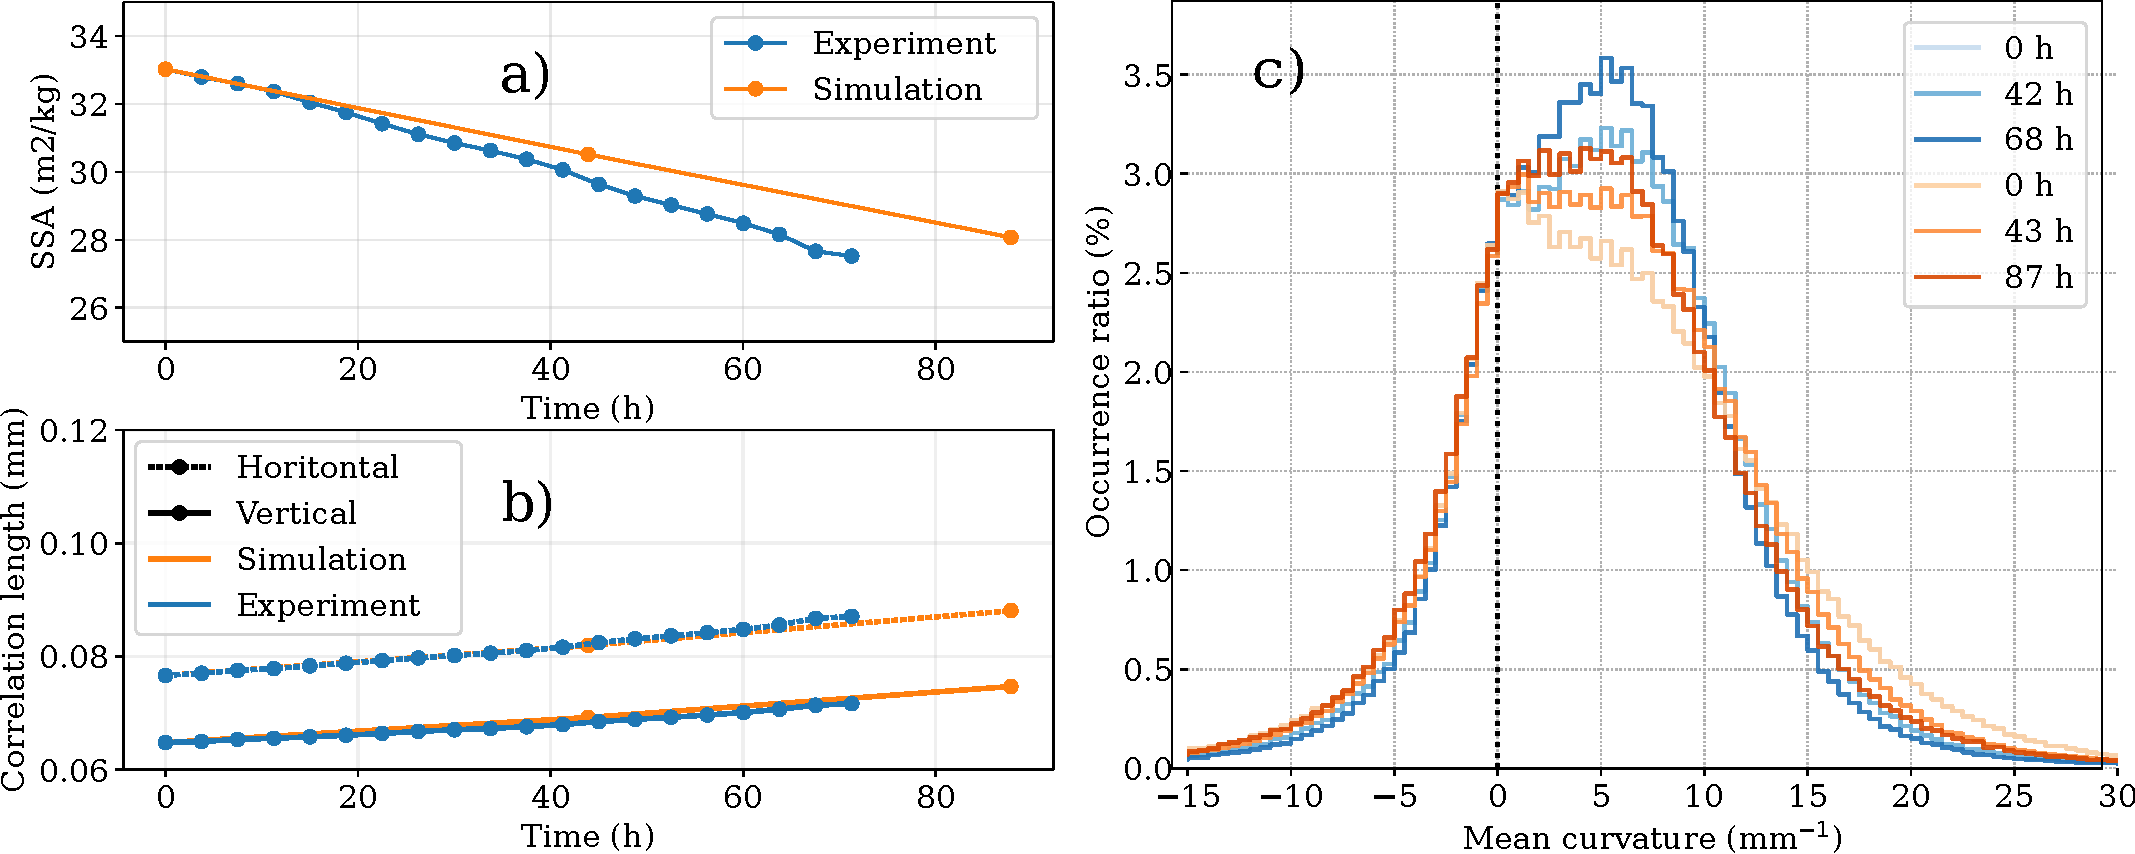
\includegraphics[width=\linewidth]{Figures/eboni_courbes_lc_ssa_histo.pdf}
    \caption{Comparison between \protect\citeA{hagenmuller_motion_2019} experimental series and simulation results. a) SSA ; b) correlation length ; c) mean curvature histograms.}
    \label{fig:eboni}
\end{figure}


\subsection{Model prediction}
\label{sec:prediction}

After considering the calibration evaluation and validation, the model is used to predict equi-temperature metamorphism effects on different snow experimental images (Table \ref{tab:series_sim}). We selected 4 3D experimental images of snow showing various features and use them as initial image in the model. The samples are I17 (DF), which present an isotropic structure with rounded shapes, TG2 (FC/DH), Grad3 (DH), and 7G9m (DH). The 3 last images underwent various temperature gradient with an effect increasingly pronounced (see Table \ref{tab:series_sim}). The simulations were performed with isothermal conditions at a temperature T = -2$^\circ$C and $\alpha = 9.8\ 10^{-4}$. It led to 4 series of 4 to 11 images simulating from 70 days to 80 days of isothermal metamorphism. This time range enables to capture the important physical evolution while remaining realistic. In Figure \ref{fig:evolutions_3D}, we see the simulated series of our 4 samples, with a perspective view of three steps for each series, and vertical slices associated to those steps.\\

\begin{figure}
    \centering
    \includegraphics[width =\linewidth]{Figures/evolution_3D_new_textepetit_courr.pdf}
    \caption{Simulated evolution 3D views and their vertical slices taken at the center of each cube.}
    \label{fig:evolutions_3D}
\end{figure}
\subsubsection{Microstructural parameters}
\begin{figure}
    \centering
    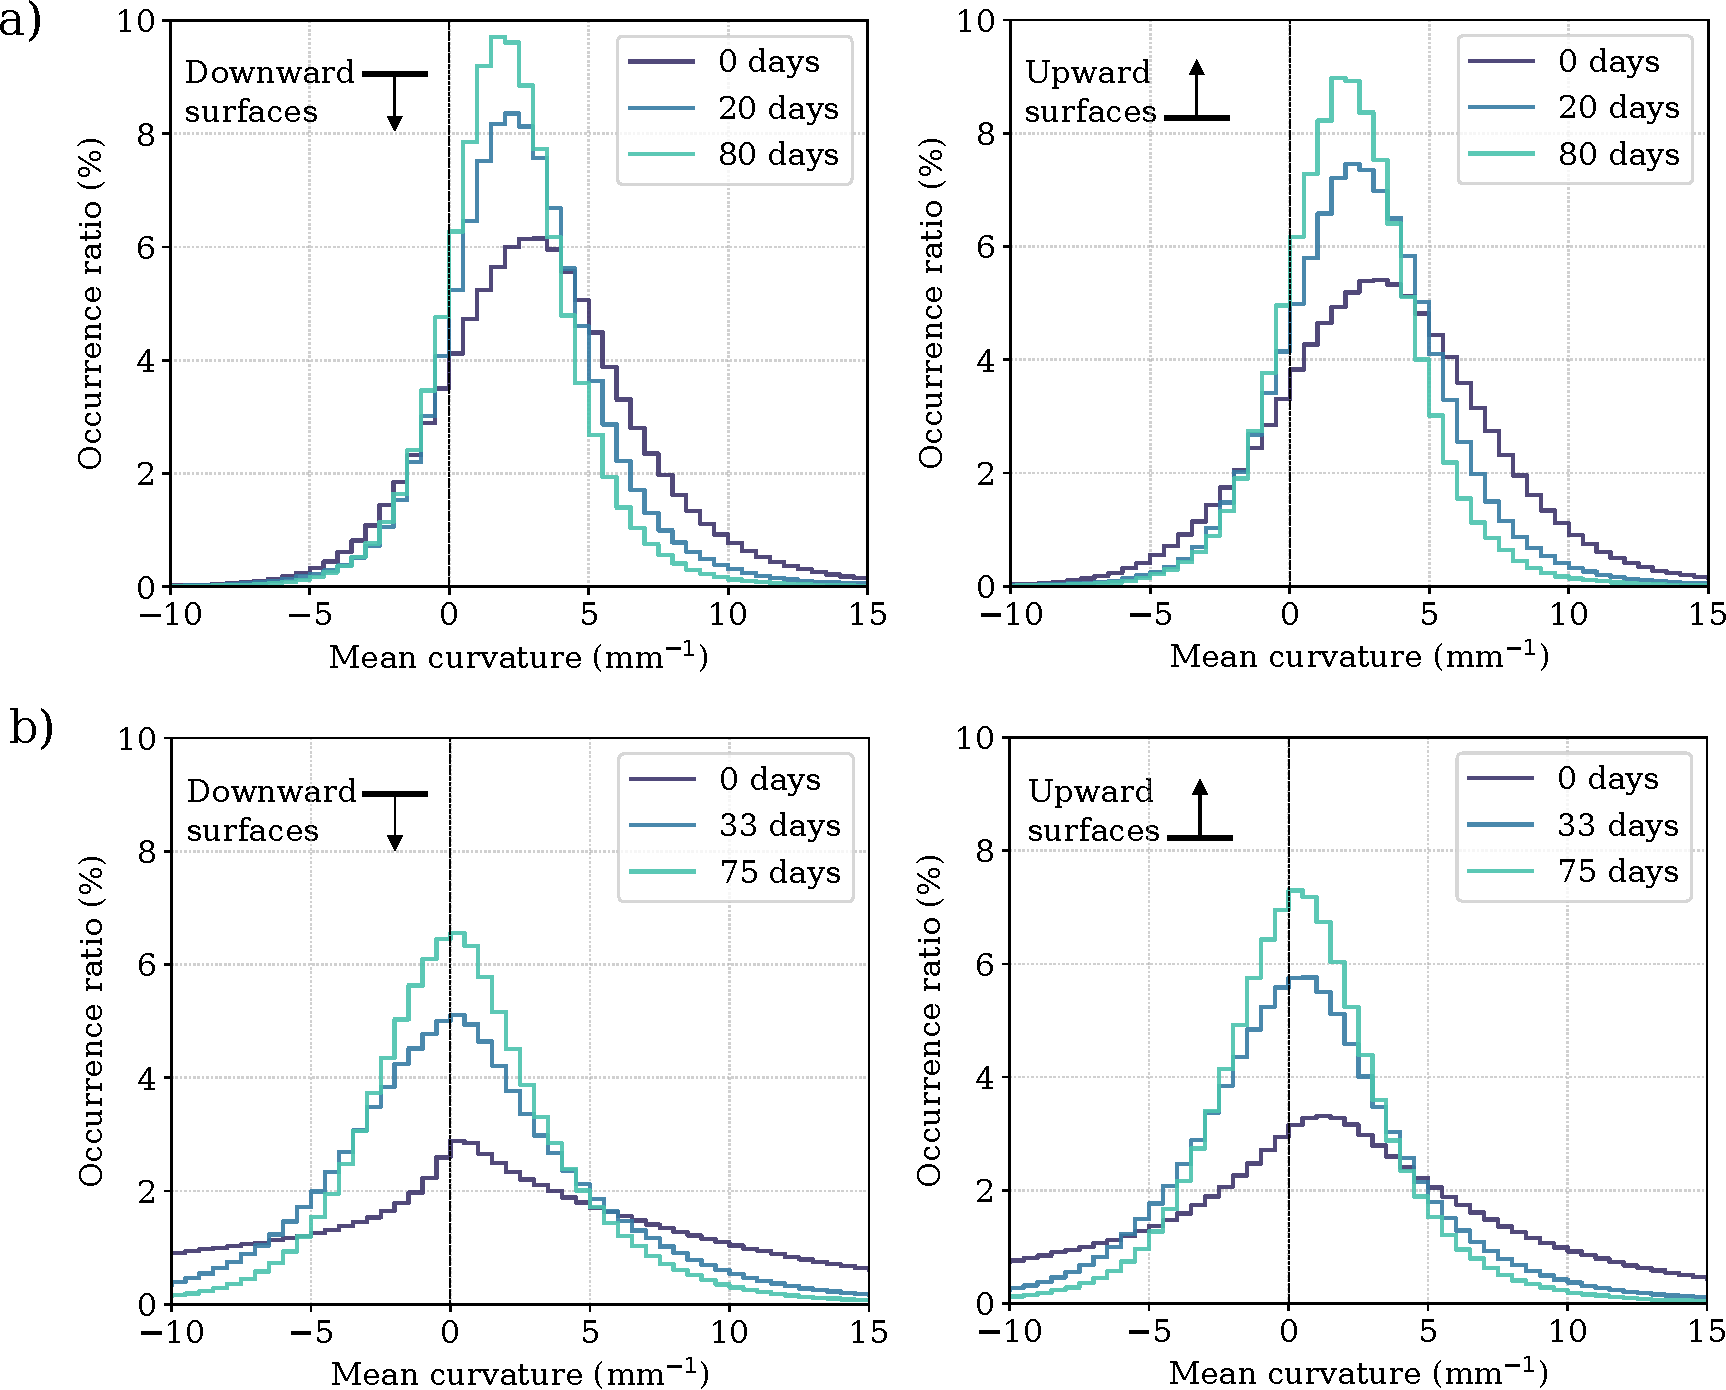
\includegraphics[width=\linewidth]{Figures/histo_i17_grad3_copie_invert.pdf}
    \caption{Time evolution of the mean curvature distribution from the downward (left) and upward (right) surfaces of I17 (a) and Grad3 (b) simulated series. Each curvature class is 0.5 mm$^{-1}$ wide.}
    \label{fig:histo_i17_grad3}
\end{figure}

In Figure \ref{fig:histo_i17_grad3}, we see the mean curvature distribution evolution for I17 (DF) and Grad3 (DH) samples (Sec. \ref{subsec:methode_physical_appli}).\\
For I17 simulated evolution (Figure \ref{fig:histo_i17_grad3}.a), the initial upward and downward distributions are similar with a peak of mean curvature located around 4 mm$^{-1}$ and an occurrence ratio of 5 \%. It shows that this sample was initially isotropic. With time, the area-averaged mean curvature decreases gradually, and the distributions are narrowing as the ice structure tend to become larger and more uniform.\\
For Grad3 evolution (Figure \ref{fig:histo_i17_grad3}.b), the initial upward and downward distributions are wider than for I17 initial sample. It can be explained by the large variety of shapes encountered in Grad3 and not in I17 that already presents homogeneous rounded shapes. For Grad3, the initial upward and downward surfaces exhibit clearly distinct distributions: the peak of mean curvature is located around 0 mm$^{-1}$ for the downward ones, and at 1.5 mm$^{-1}$ for the upward ones. The near 0 downward distribution depicts the plane surfaces that are typically found downward a depth hoar structure, unlike the upward outlook that presents more rounded shapes. With time, the area-averaged mean curvature stays very low but the distributions are narrowing (approx. 7 \% occurrence ratio), showing the same trend as I17.\\

\begin{figure}
    \centering
    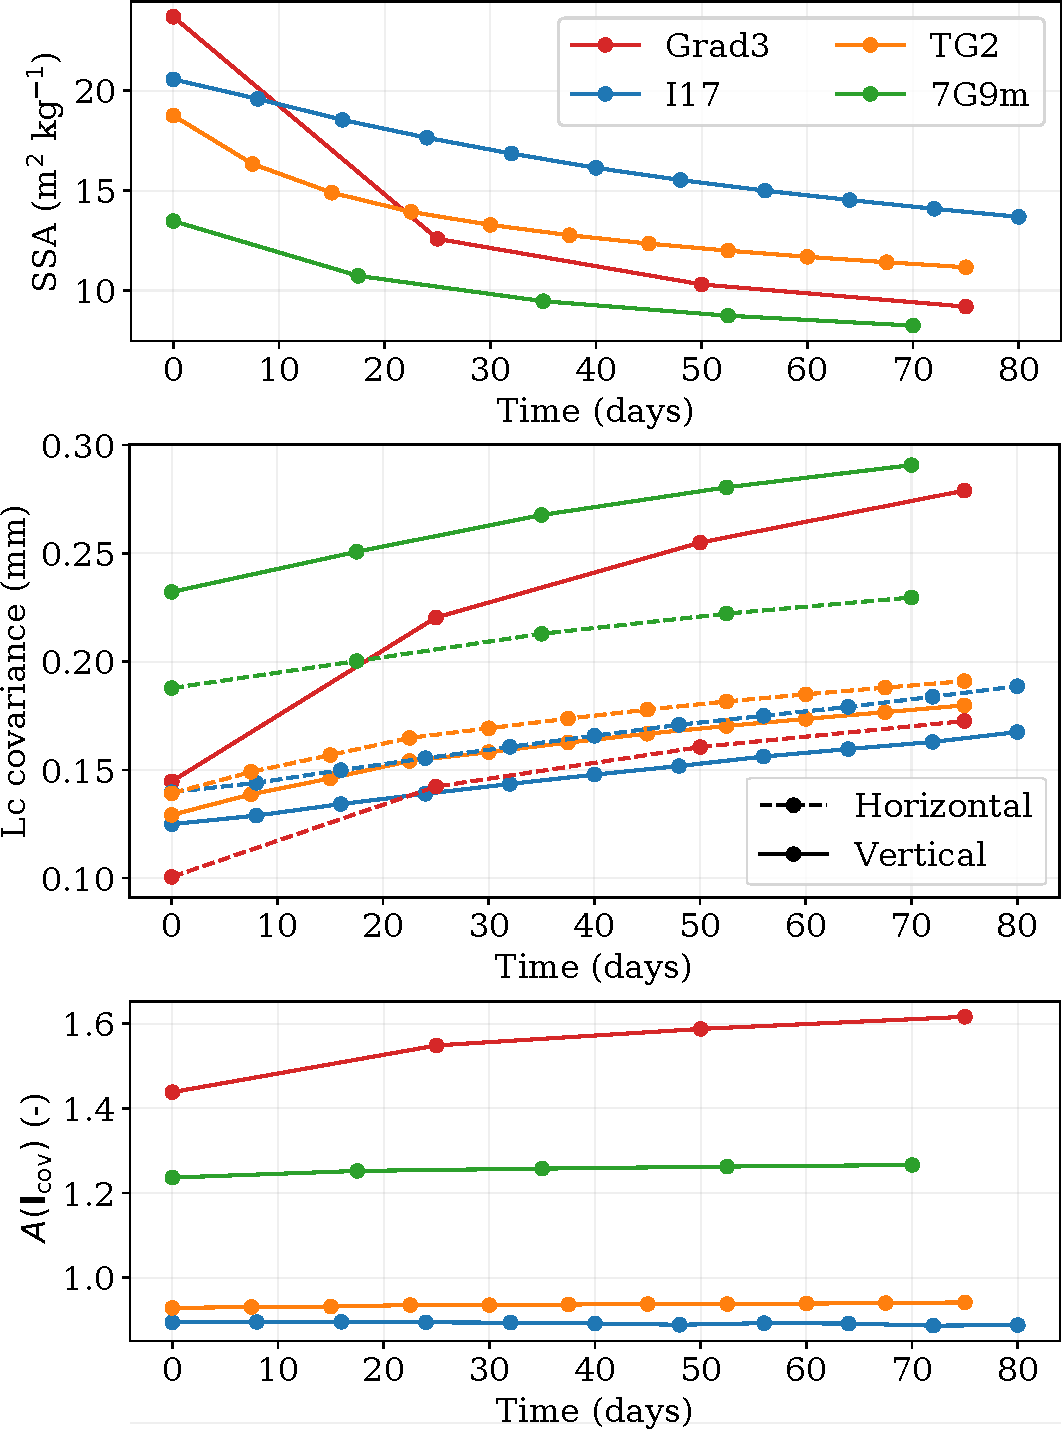
\includegraphics[width=0.6\linewidth]{Figures/4_images_microstructure.pdf}
    \caption{Microstructural parameters of the simulated series.}
    \label{fig:4_images_microstruct}
\end{figure}
Figure \ref{fig:4_images_microstruct} shows the microstructural parameters of our 4 simulated series. For the SSA graph, we see an exponential decrease for each image, which matches with ETM experiments and similar models \cite{vetter_simulating_2010, kaempfer_observation_2007}. Each series shows different decreasing rate and shape, ranging from Grad3 with an exponential decrease of 23.7 to 9.2 m$^2$ kg$^{-1}$ to the almost linear slope of I17 curve from 20.6 to 13.7 m$^2$ kg$^{-1}$. This difference in decrease rate  is due to the initial microstructure. Grad3 shows a high initial SSA value, with sharp edges and facets that evolve quickly under isothermal conditions, unlike the sample I17 that presents rounded shapes in its initial stage.
The covariance length evolution shows the characteristic increase of the ETM, reflecting the growth of snow grains and pores \cite{lowe2011interfacial, calonne_study_2014}. Different evolution rates are again observed, from an increase of 0.05 mm for I17 to 0.09 mm for Grad3. Finally, looking at the anisotropy ratio evolution provides surprising results. The samples I17 and TG2 presenting a rather isotropic structure, with ratio close to 1, show no changes over time. Samples initially anisotropic, however, show an increase of their anisotropy, as Grad3 increasing from 1.44 to 1.62 through the simulation and, in a lesser way, 7G9m ranging from 1.24 to 1.27. By the end of the simulations, Grad3 covariance length is about two times larger in the vertical direction than in the horizontal direction. This increase in anisotropy can also be seen in the slices and 3D images (Fig. \ref{fig:evolutions_3D}): the initial vertically elongated structure is strengthening with the growing of vertical columns. This is an interesting result because one could think that a sample presenting a strong anisotropy would tend to lose it for the benefit of a more isotropic structure under the effect of a long equi-temperature exposure.



\subsubsection{Macroscale transport properties}

In this section we present 3D estimates of macroscopic transport properties (Sec. \ref{subsec:methode_physical_appli}) calculated on the simulated series predicting ETM on a large range of microstructures (Sec. \ref{sec:prediction}). The estimations are displayed along with isotropic models based on simplified microstructures (effective coefficient of diffusion \textbf{D}) and current regressions (thermal conductivity \textbf{k} and permeability \textbf{K}). For the conductivity we use the regression of \citeA{calonne_numerical_2011} obtained using images of snow spanning a wide range of seasonal snow types. The self-consistent estimate of diffusion for spherical inclusions $D_{\mathrm{SC}}$ from \citeA{calonne_macroscopic_2014} is shown for the effective coefficient of diffusion, and the regression from \citeA{calonne_3D_2012} is used for the normalized permeability: \\
\begin{subequations}
\begin{align}
k_{\mathrm{Calonne\ 2011}}=2.5 \times 10^{-6} \rho_{\mathrm{s}}^{2}-1.23 \times 10^{-4} \rho_{\mathrm{s}}+0.024\end{align}
\begin{align}
D_{\mathrm{SC}} = 1 - \frac{3\rho_s}{2\rho_i}
\end{align}
\begin{align}
K_{\mathrm{Calonne\ 2012}}=(3.0 \pm 0.3)\ \exp \left(\left(-0.0130 \pm 0.0003\right) \rho_{\mathrm{s}}\right)
\end{align}
\end{subequations}

The Figure \ref{fig:Tplot} shows estimates of conductivity, effective coefficient of diffusion and permeability plotted as a function of the density for each image of our simulated series. To show the structural anisotropy of the samples, the tips and horizontal bars of the ``T" markers represent respectively the vertical and horizontal components. The arrows indicate the evolution direction of the simulated series in time. The relative change between the initial sample and the last step of the simulation $\tau$ is indicated in the legends for each property.
% , calculated for the horizontal component ($\tau_{x y}$) and for the vertical component ($\tau_{z}$) are indicated in the legends for each property.\\
 
When looking at Figure \ref{fig:Tplot}, the series show an evolution along the density axis, with a maximum of 10 kg m$^{-3}$ (3\%) increase for the TG2 series and a minimum of 4 kg m$^{-3}$ (1\%) for the Grad3 series. As the model is supposed to operate at constant density, this rather small density changes are artefacts. They could be caused by the images resolution, too high in comparison with the small elements of the snow images, causing inaccurate loss or gain of ice voxels in the model. We suppose that the increase in density is however distributed on the whole sample such that the arising images have a realistic microstructure (Sec. \ref{sec:disc}).

The temporal evolution of the different series in terms of the macroscale properties and of the density, represented by the arrows and by the relative changes $\tau$, mostly follow the reference parameterizations. This shows that the predicted ETM is in overall good agreement with the expected evolution of those macroscopic properties. 

Grad3 and 7G9m evolution in \textbf{D} are the only series estimates evolving in opposition with the reference parameterization. Those trends can be interpreted with the influence of the microstructure: the Figure 9 of \citeA{calonne_macroscopic_2014} display the normalized effective vapor diffusion versus snow density with the model $D_{\mathrm{SC}}$ and different measurements. We observe that when the density increases, $D$ essentially decreases with a given dispersion. When looking in more details, we also observe that for a given density, effective vapor diffusion is smaller for depth hoar samples than for faceted crystals and for rounded grains samples. As Grad3 and 7G9m samples evolve from depth hoar to more rounded shapes (Figure \ref{fig:evolutions_3D}) while increasing in density, the changes in microstructure and in density are in opposition and the microstructure influence could overcome the increase in density. \\
This microstructure influence is also present for the permeability, as seen in Figure 1 of \citeA{calonne_3D_2012}. In this figure, the permeability regression decreases when the density increases, but at a given density, depth hoar seems to have higher permeability than faceted crystals or rounded grains. For Grad3 and 7G9m, the microstructure and the density evolution leads to a decreasing permeability.\\
For the thermal conductivity, the microstructure impact does not seem to be that distinct as seen in the Figure 1 of \citeA{calonne_numerical_2011}.


\begin{figure}
    \centering
    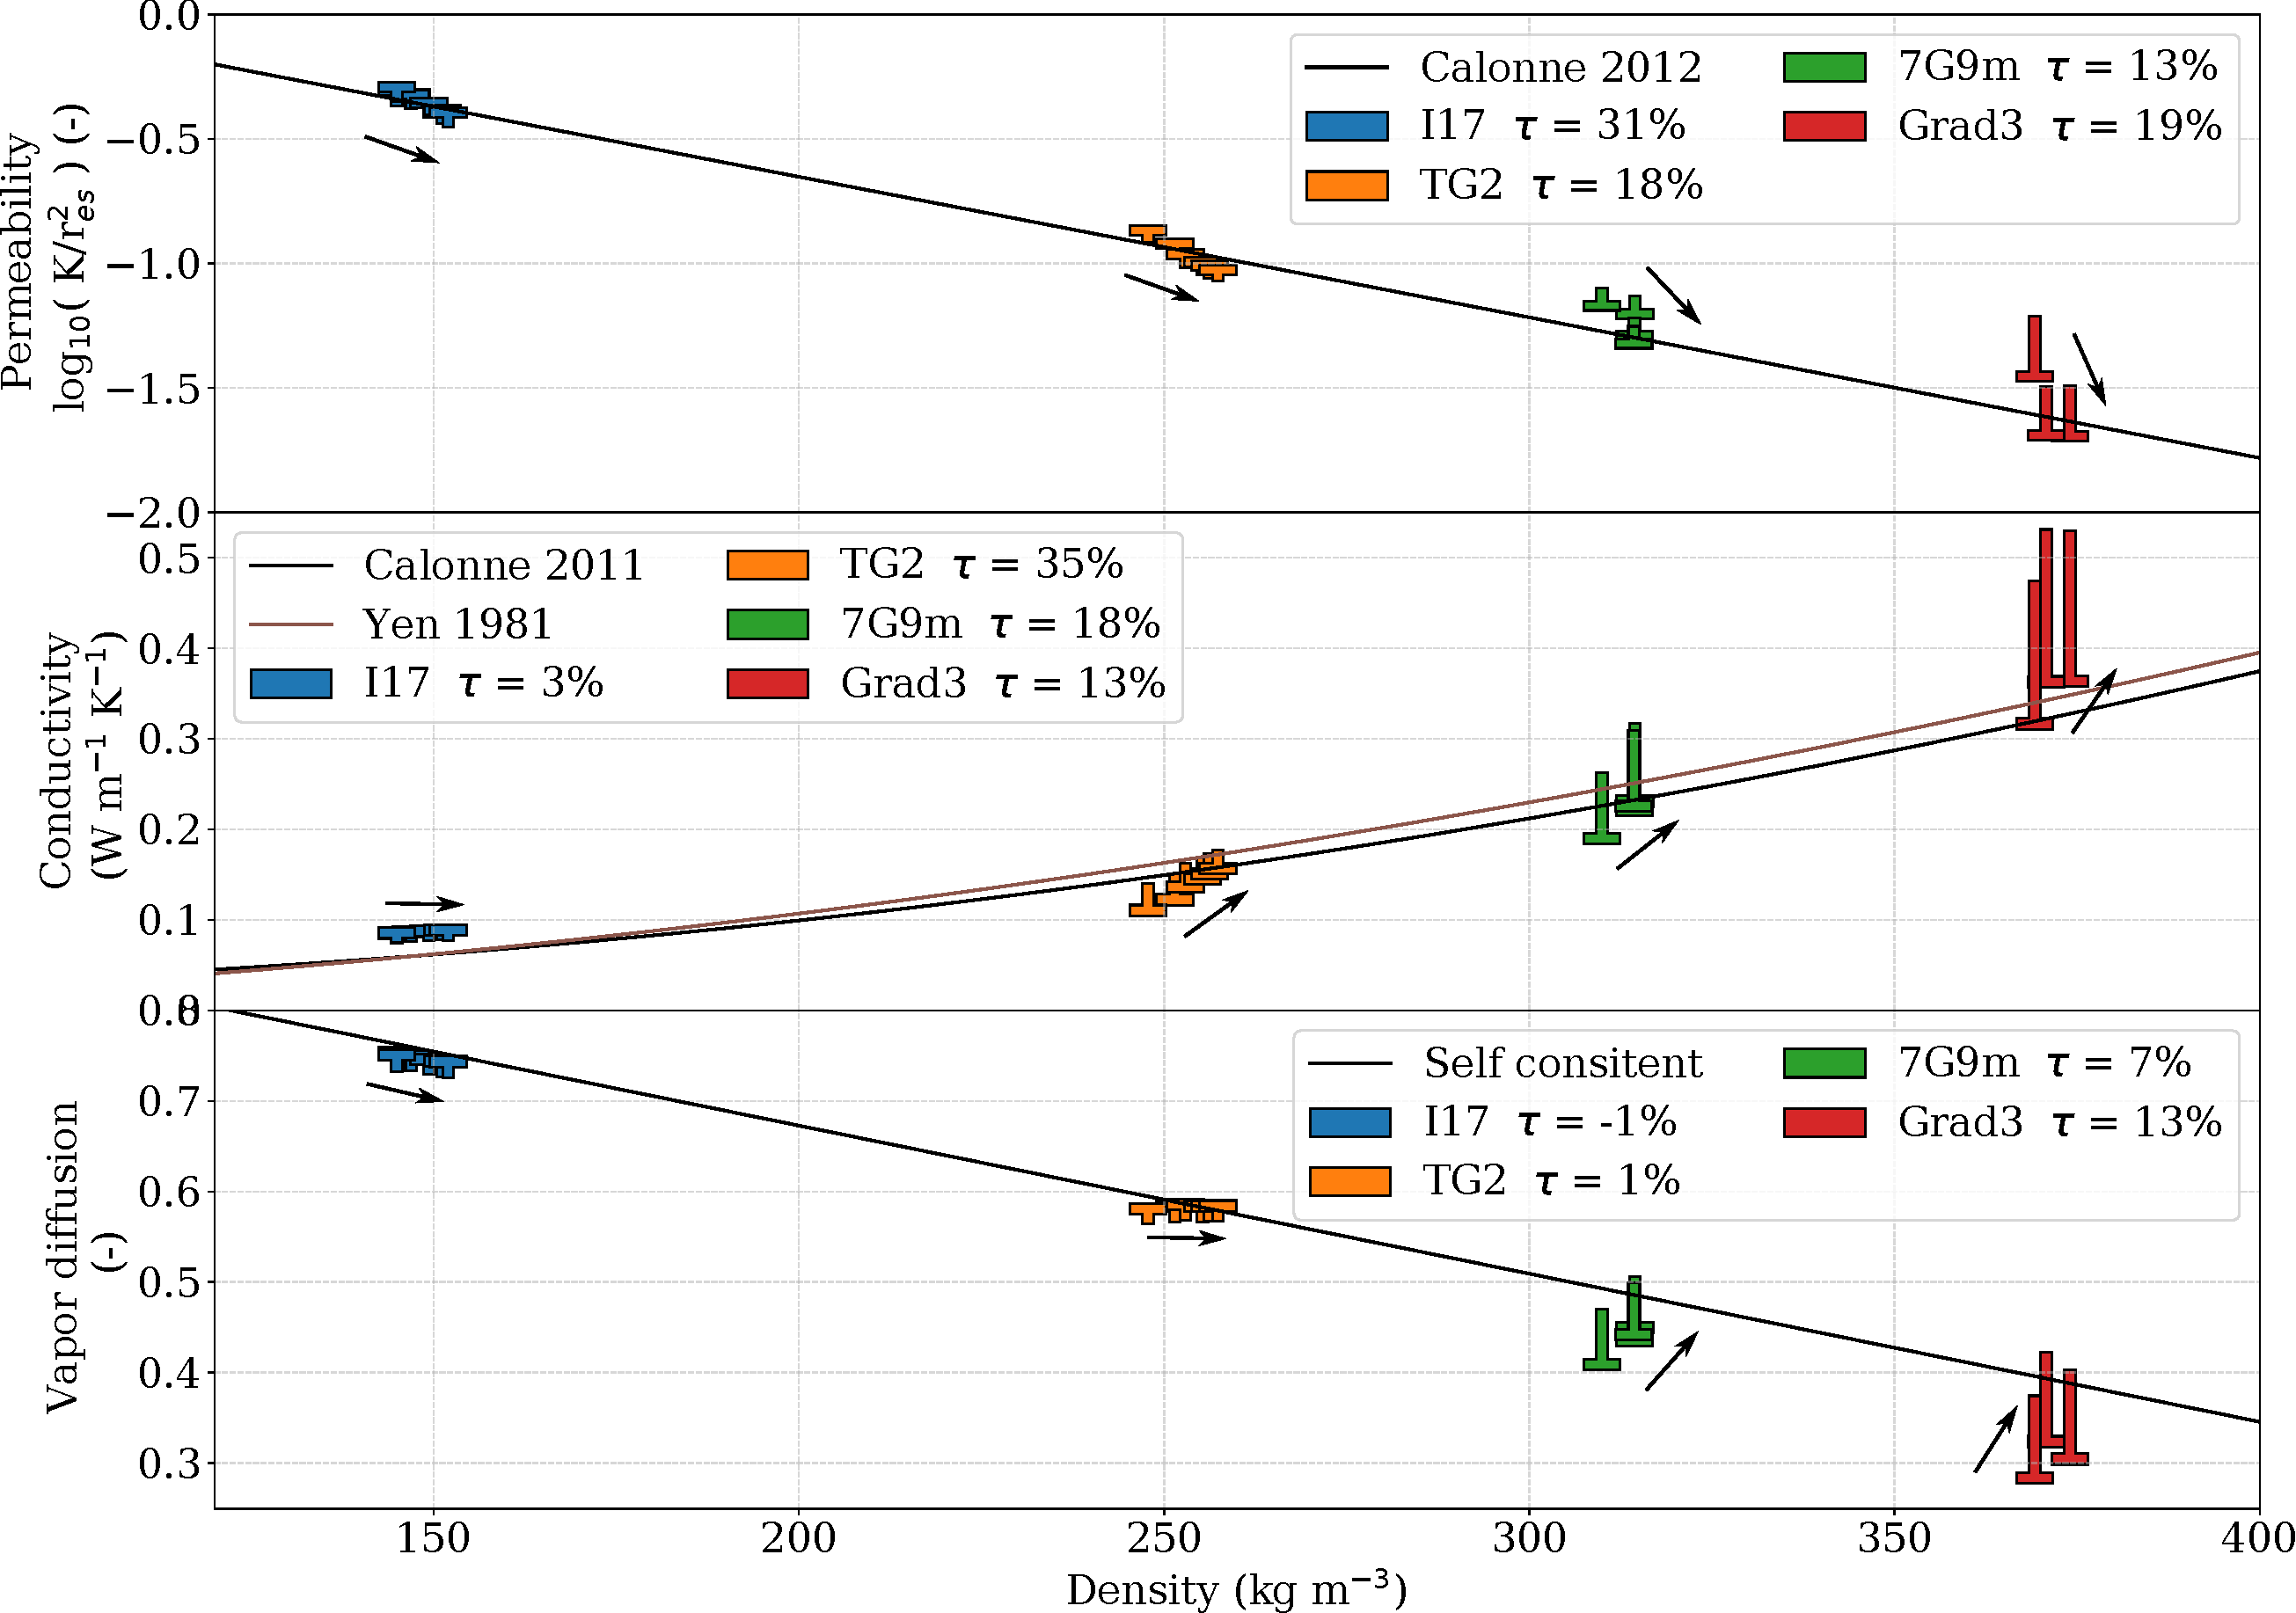
\includegraphics[width=\linewidth]{Figures/tplot_all_arrows.pdf}
    \caption{Effective thermal conductivity, normalized effective vapor diffusion and normalized permeability as a function of density.}
    \label{fig:Tplot}
\end{figure}


\section{Discussion}
\label{sec:disc}

This work provides a new simple curvature driven sublimation-deposition model representing ETM applicable on real 3D tomographic images. This optimized model has been calibrated and validated using experimental ETM series, and used for metamorphism prediction on a large range of microstructures by characterizing the images using numerous microstructural and macroscale transport properties.

% The Snow-3D model is reliable for modeling ETM to some extent: it only consider sublimation-deposition, setting settling and water vapor transport processes aside and constraining the choice of the input microstructures.

Having the results in mind, it is worth while discussing the models artefacts in some more details. 
% density increase ------------
For our 4 simulated series, we observed a moderate increase in density in Figure \ref{fig:Tplot} whereas the model does not simulate changes in density. This change is thus an artefact that contradicts mass conservation. A likely cause of this artefact seems to be the image resolution. In Figure \ref{fig:cubes}, we run the model on four different images: a cube surrounded by air with a size of 40$^3$ voxels ; the same cube with a size of 400$^3$ voxels ; the complement of the cube - a cube of air surrounded by ice - with a size of 40$^3$ voxels and the same image at 400$^3$ voxels. The idea is to test the simulated density evolution for different resolution and shapes, with an image presenting convex shapes (the cube) and with one presenting concave shapes (the cube complement). Those shapes have been created such as the ratio of the object length over the voxel size is similar to the one of the data of Figure \ref{fig:Tplot}. We see clearly in the graph that for a fine resolution, the density is stable in time, whereas for a coarser resolution, the density has an erratic progression, with loss and gain of about 40 kg m$^{-3}$. Furthermore, the ratio between the elements size and the resolution gets larger from I17, to TG2 to Grad3 and to 7G9m, as the density changes gets smaller. In our data, the maximum density increase is of 3\% for the TG2 series. It is however within the precision range of snow density measurements such as the box cutter that have a precision of 5\% \cite{proksch2016intercomparison}. Moreover, the settling process has an important role in ETM. For example in \citeA{flin_three-dimensional_2004} the density increases of 95 kg m$^{-3}$ in 80 days. Thus, the artefact is small in comparison with the measurement precision and the observed settling, and it enables to investigate the model on images with different snow densities.\\
\begin{figure}
    \centering
    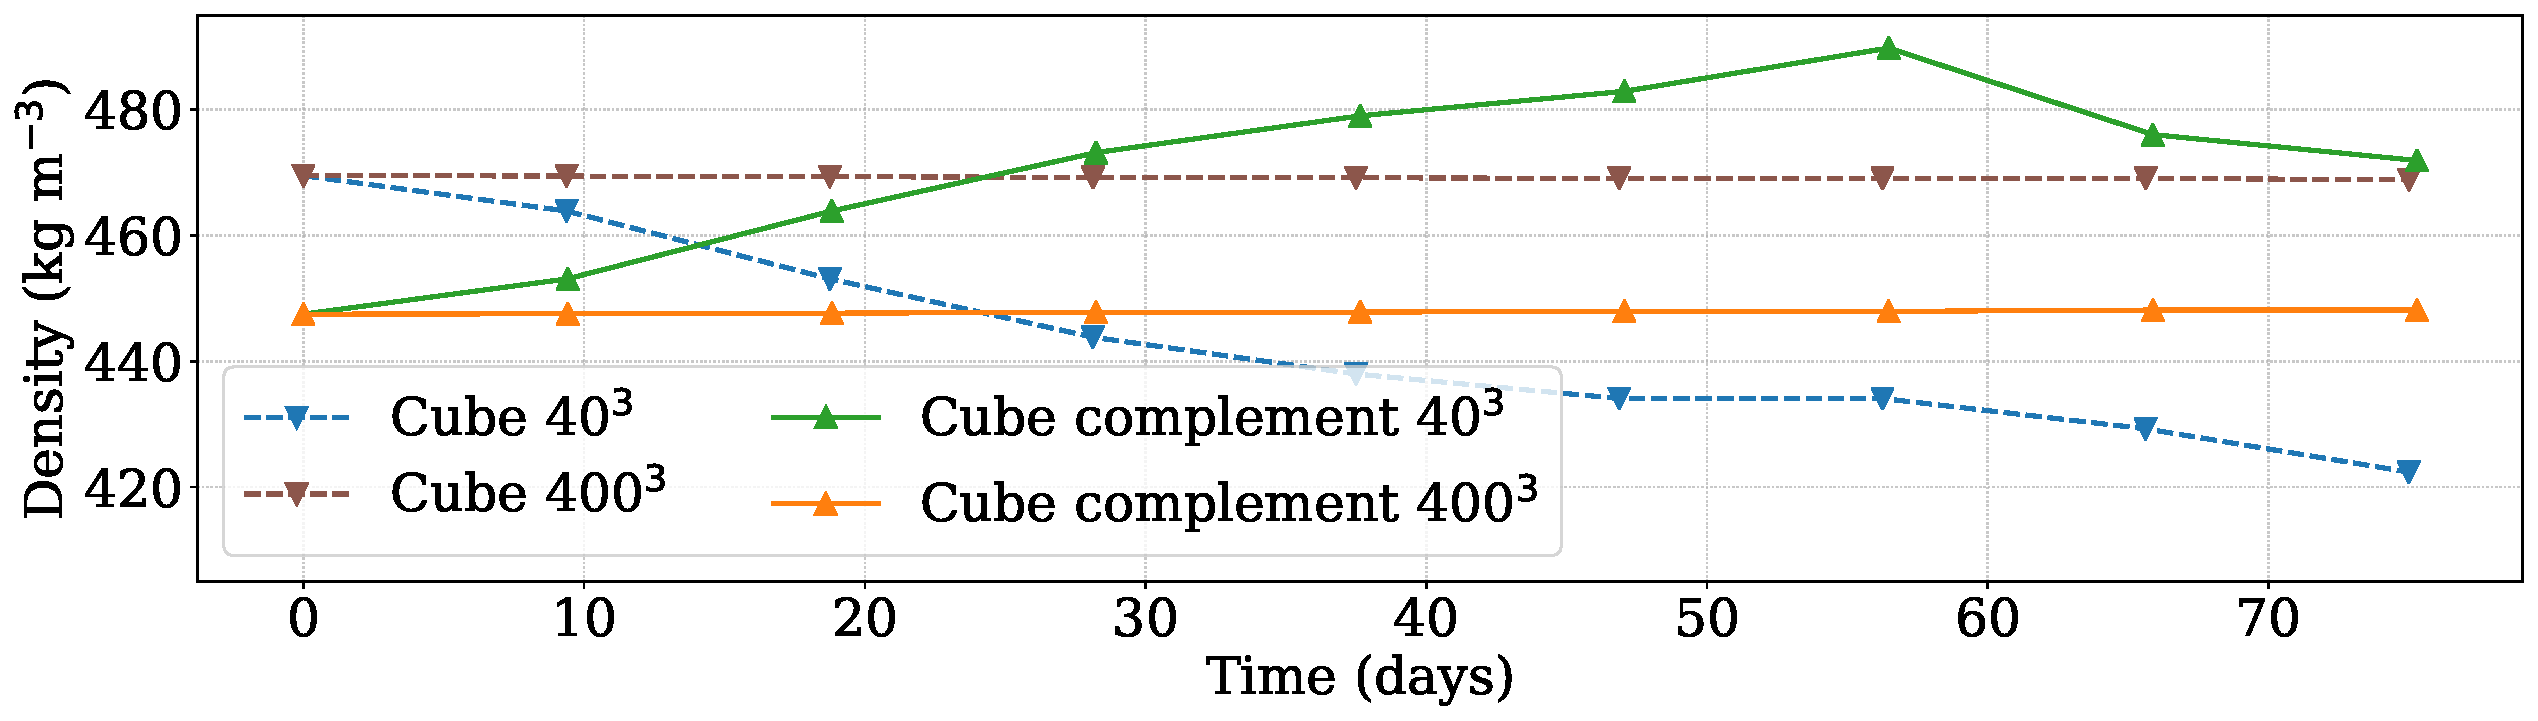
\includegraphics[width=0.9\linewidth]{Figures/cubes_compl_density_propre.pdf}
    \caption{Influence of the image resolution on the modeled density evolution: example of a cube surrounded by air and its complementary image.}
    \label{fig:cubes}
\end{figure}
% ---------------------------- 1ere itération
In Figure \ref{fig:Tplot} we also see a gap between the first image of each series, which is the experimental one, and the simulated ones. This gap can be caused by the first step of the algorithm, which modify the image to conform it to the model constraints.\\
% -----------------------------
% Calibration et validation -------------
Other points worth discussing are the calibration and validation. The condensation coefficient $\alpha$ has been approximated by an isotropic constant value. This hypothesis has however never been verified and $\alpha$ seems to have numerous dependencies. For example, \citeA{libbrecht2019snow} highlighted dependencies in temperature, supersaturation and crystalline orientation. He measured basal and prismatic $\alpha$ on growing snow crystal, with results between $10^{-3}$ and $10^{-1}$.
In our calibration process, the $\alpha$ parameter has been determined using an experimental series of \citeA{flin_three-dimensional_2004} obtained at -2$^\circ$C. In view of $\alpha$ complex dependencies, its calibrated value can incorporate non-modeled experimental conditions (temperature variations, vapor diffusion...).
To test and validate the calibration, we used the equi-temperature time series of \citeA{hagenmuller_motion_2019}, also realized at -2$^\circ$C. %In terms of SSA, the simulated results using the calibrated $\alpha$ and the experimental SSA are in the same order of magnitude.%, but one can notice that \citeA{hagenmuller_motion_2019} experimental SSA does not really follow the expected decreasing exponential curve. 
As the experimental time series is very short compared to \citeA{flin_three-dimensional_2004} (3 days versus 28 days used), the comparison with the microstructural properties is relatively weak and would benefit of a comparison with a longer independent series of ETM. %For example, the RMSE of the SSA could significantly increase if the SSA followed the same trend for a longer period.
%This effect is however balanced by the comparison of experimental and simulated covariance lengths, showing a very good fit. It shows that even if the SSA curves does not match perfectly, the microstructural evolution under equi-temperature conditions is rather well simulated.
% ------------ Prediction

Finally, concerning the ETM prediction, the notable result is the enhancement of structural anisotropy for the very anisotropic depth hoar sample Grad3. The Grad3 experimental sample (DH) has a particular structure: it presents a dense structure with many intricate angular shapes. On a larger scale, the sample seems to be organized into vertical shapes. With ETM the general smoothing could remove small shapes to let the general structure appear with the formation of wide vertical columns, increasing the value of the structural anisotropy. A conservation of the anisotropy is also observed for 7G9m, without significant increase. One can still question if this result is particular to this only sample or if it can be generalized for any strongly anisotropic sample. 

\section{Conclusion}
\label{sec:conclusion}

% The application of \citeA{bretin_phase-field_2019} model to the isothermal metamorphism of snow by the condensation-sublimation process was investigated. The model has been calibrated through the only condensation coefficient $\alpha$ parameter using the SSA of the experimental series of \cite{flin_three-dimensional_2004}. The resulting value is $\alpha = ( 9.8 \pm 0.70) 10^{-4}$. An evaluation of this calibration has been made using the independent experimental series of \cite{hagenmuller_motion_2019} by looking at microstructural properties such as the SSA, the covariance length and the structural anisotropy. As this validation gave very encouraging results, the model Snow3D was used to model isothermal metamorphism on a representative range of microstructures using experimental samples. On the simulated time series, we analyzed microstructural parameters (SSA, $\mathrm{l_{cov}}$, $A_{\mathrm{l_{cov}}}$) and physical transport properties (thermal conductivity, diffusivity and permeability). The comparison of the simulations physical properties and the current related parameterizations shows that the model operates properly for different densities. The microstructural results exhibit the expected global variations for the SSA and covariance length. For the very anisotropic sample Grad3, the structural anisotropy increases with time, leading to a vertical columnar structure. It questions the idea that isotropic conditions could tend to remove the snow structure anisotropy. This model is a step forward for modeling ETM. Future studies will focus on implementing the settling process and water vapor transport in pores, as well on studying the condensation coefficient depending on various parameters such as the temperature.  

The application of \citeA{bretin_phase-field_2019} model to snow ETM described by the condensation-sublimation process is investigated. The model is calibrated to experimental data at – 2°C by fitting the SSA of the series from \citeA{flin_three-dimensional_2004} to the simulation. A single value of the condensation coefficient $\alpha$ is derived: $\alpha = ( 9.8 \pm 0.7) 10^{-4}$. The calibrated model is then evaluated with the independent experimental series of \citeA{hagenmuller_motion_2019} by looking at microstructural properties such as the SSA, the covariance length, the structural anisotropy and the mean curvature. As this evaluation raises very encouraging results, the model Snow-3D is used to model ETM on four different snow microstructures from experimental samples. The four simulated time series are used to analyze microstructural parameters (SSA, covariance length, structural anisotropy) and physical effective transport properties (thermal conductivity, vapor diffusivity and permeability). This results are in good agreement with current models and regressions. They also exhibit the influence of the microstructure on micro-scale (structural anisotropy) and macro-scale (effective coefficient of diffusion) phenomenon. For example, we observe an enhancement of the structural anisotropy in the case of initially anisotropic microstructures. It questions the idea that isotropic conditions tends to remove the snow structure anisotropy. This model is a step forward for modeling ETM at the pore scale. Future studies will focus on implementing the settling process and water vapor transport in pores, as well on studying the condensation coefficient depending on various parameters such as the temperature.  

\acknowledgments
The 3SR lab is part of the Labex Tec 21 (investissements d'Avenir, Grand Agreement ANR-11-LABX-0030). CNRM/CEN is part of Labex OSUG@2020 (Investissements d'Avenir, Grand ANR-10-LABX-0056).
%TC:endignore
\bibliography{Snow3D}




\end{document}


